\documentclass[twoside]{book}

% Packages required by doxygen
\usepackage{fixltx2e}
\usepackage{calc}
\usepackage{doxygen}
\usepackage{graphicx}
\usepackage[utf8]{inputenc}
\usepackage{makeidx}
\usepackage{multicol}
\usepackage{multirow}
\PassOptionsToPackage{warn}{textcomp}
\usepackage{textcomp}
\usepackage[nointegrals]{wasysym}
\usepackage[table]{xcolor}

% Font selection
\usepackage[T1]{fontenc}
\usepackage{mathptmx}
\usepackage[scaled=.90]{helvet}
\usepackage{courier}
\usepackage{amssymb}
\usepackage{sectsty}
\renewcommand{\familydefault}{\sfdefault}
\allsectionsfont{%
  \fontseries{bc}\selectfont%
  \color{darkgray}%
}
\renewcommand{\DoxyLabelFont}{%
  \fontseries{bc}\selectfont%
  \color{darkgray}%
}
\newcommand{\+}{\discretionary{\mbox{\scriptsize$\hookleftarrow$}}{}{}}

% Page & text layout
\usepackage{geometry}
\geometry{%
  a4paper,%
  top=2.5cm,%
  bottom=2.5cm,%
  left=2.5cm,%
  right=2.5cm%
}
\tolerance=750
\hfuzz=15pt
\hbadness=750
\setlength{\emergencystretch}{15pt}
\setlength{\parindent}{0cm}
\setlength{\parskip}{0.2cm}
\makeatletter
\renewcommand{\paragraph}{%
  \@startsection{paragraph}{4}{0ex}{-1.0ex}{1.0ex}{%
    \normalfont\normalsize\bfseries\SS@parafont%
  }%
}
\renewcommand{\subparagraph}{%
  \@startsection{subparagraph}{5}{0ex}{-1.0ex}{1.0ex}{%
    \normalfont\normalsize\bfseries\SS@subparafont%
  }%
}
\makeatother

% Headers & footers
\usepackage{fancyhdr}
\pagestyle{fancyplain}
\fancyhead[LE]{\fancyplain{}{\bfseries\thepage}}
\fancyhead[CE]{\fancyplain{}{}}
\fancyhead[RE]{\fancyplain{}{\bfseries\leftmark}}
\fancyhead[LO]{\fancyplain{}{\bfseries\rightmark}}
\fancyhead[CO]{\fancyplain{}{}}
\fancyhead[RO]{\fancyplain{}{\bfseries\thepage}}
\fancyfoot[LE]{\fancyplain{}{}}
\fancyfoot[CE]{\fancyplain{}{}}
\fancyfoot[RE]{\fancyplain{}{\bfseries\scriptsize Generated on Thu Mar 30 2017 14\+:37\+:28 for Project Feast Documentation by Doxygen }}
\fancyfoot[LO]{\fancyplain{}{\bfseries\scriptsize Generated on Thu Mar 30 2017 14\+:37\+:28 for Project Feast Documentation by Doxygen }}
\fancyfoot[CO]{\fancyplain{}{}}
\fancyfoot[RO]{\fancyplain{}{}}
\renewcommand{\footrulewidth}{0.4pt}
\renewcommand{\chaptermark}[1]{%
  \markboth{#1}{}%
}
\renewcommand{\sectionmark}[1]{%
  \markright{\thesection\ #1}%
}

% Indices & bibliography
\usepackage{natbib}
\usepackage[titles]{tocloft}
\setcounter{tocdepth}{3}
\setcounter{secnumdepth}{5}
\makeindex

% Hyperlinks (required, but should be loaded last)
\usepackage{ifpdf}
\ifpdf
  \usepackage[pdftex,pagebackref=true]{hyperref}
\else
  \usepackage[ps2pdf,pagebackref=true]{hyperref}
\fi
\hypersetup{%
  colorlinks=true,%
  linkcolor=blue,%
  citecolor=blue,%
  unicode%
}

% Custom commands
\newcommand{\clearemptydoublepage}{%
  \newpage{\pagestyle{empty}\cleardoublepage}%
}


%===== C O N T E N T S =====

\begin{document}

% Titlepage & ToC
\hypersetup{pageanchor=false,
             bookmarks=true,
             bookmarksnumbered=true,
             pdfencoding=unicode
            }
\pagenumbering{roman}
\begin{titlepage}
\vspace*{7cm}
\begin{center}%
{\Large Project Feast Documentation }\\
\vspace*{1cm}
{\large Generated by Doxygen 1.8.8}\\
\vspace*{0.5cm}
{\small Thu Mar 30 2017 14:37:28}\\
\end{center}
\end{titlepage}
\clearemptydoublepage
\tableofcontents
\clearemptydoublepage
\pagenumbering{arabic}
\hypersetup{pageanchor=true}

%--- Begin generated contents ---
\chapter{Hierarchical Index}
\section{Class Hierarchy}
This inheritance list is sorted roughly, but not completely, alphabetically\+:\begin{DoxyCompactList}
\item \contentsline{section}{Body\+Part}{\pageref{class_body_part}}{}
\item \contentsline{section}{Enemy}{\pageref{class_enemy}}{}
\item \contentsline{section}{Enemy\+Manager}{\pageref{class_enemy_manager}}{}
\item \contentsline{section}{Entity\+Test}{\pageref{class_entity_test}}{}
\item Frame\+Listener\begin{DoxyCompactList}
\item \contentsline{section}{Main}{\pageref{class_main}}{}
\end{DoxyCompactList}
\item \contentsline{section}{Main\+Camera}{\pageref{class_main_camera}}{}
\item \contentsline{section}{Matrix4}{\pageref{class_matrix4}}{}
\item \contentsline{section}{Matth}{\pageref{class_matth}}{}
\item \contentsline{section}{Player}{\pageref{class_player}}{}
\item Singleton\begin{DoxyCompactList}
\item \contentsline{section}{Game\+Manager}{\pageref{class_game_manager}}{}
\end{DoxyCompactList}
\item \contentsline{section}{Vector3}{\pageref{class_vector3}}{}
\item Window\+Event\+Listener\begin{DoxyCompactList}
\item \contentsline{section}{Input\+Manager}{\pageref{class_input_manager}}{}
\item \contentsline{section}{Main}{\pageref{class_main}}{}
\end{DoxyCompactList}
\end{DoxyCompactList}

\chapter{Class Index}
\section{Class List}
Here are the classes, structs, unions and interfaces with brief descriptions\+:\begin{DoxyCompactList}
\item\contentsline{section}{\hyperlink{class_body_part}{Body\+Part} }{\pageref{class_body_part}}{}
\item\contentsline{section}{\hyperlink{class_enemy}{Enemy} }{\pageref{class_enemy}}{}
\item\contentsline{section}{\hyperlink{class_enemy_manager}{Enemy\+Manager} }{\pageref{class_enemy_manager}}{}
\item\contentsline{section}{\hyperlink{class_entity_test}{Entity\+Test} }{\pageref{class_entity_test}}{}
\item\contentsline{section}{\hyperlink{class_game_manager}{Game\+Manager} }{\pageref{class_game_manager}}{}
\item\contentsline{section}{\hyperlink{class_input_manager}{Input\+Manager} }{\pageref{class_input_manager}}{}
\item\contentsline{section}{\hyperlink{class_main}{Main} }{\pageref{class_main}}{}
\item\contentsline{section}{\hyperlink{class_main_camera}{Main\+Camera} }{\pageref{class_main_camera}}{}
\item\contentsline{section}{\hyperlink{class_matth}{Matth} }{\pageref{class_matth}}{}
\item\contentsline{section}{\hyperlink{class_player}{Player} }{\pageref{class_player}}{}
\end{DoxyCompactList}

\chapter{Class Documentation}
\hypertarget{class_body_part}{}\section{Body\+Part Class Reference}
\label{class_body_part}\index{Body\+Part@{Body\+Part}}
\subsection*{Public Member Functions}
\begin{DoxyCompactItemize}
\item 
\hypertarget{class_body_part_afb8155ab202d20a855df83883a25b7c8}{}void {\bfseries Spawn} ()\label{class_body_part_afb8155ab202d20a855df83883a25b7c8}

\end{DoxyCompactItemize}


The documentation for this class was generated from the following files\+:\begin{DoxyCompactItemize}
\item 
Body\+Part.\+h\item 
Body\+Part.\+cpp\end{DoxyCompactItemize}

\hypertarget{class_enemy}{}\section{Enemy Class Reference}
\label{class_enemy}\index{Enemy@{Enemy}}
\subsection*{Public Member Functions}
\begin{DoxyCompactItemize}
\item 
\hypertarget{class_enemy_aa01a1c40c682cc7c36995f26533bcb56}{}void {\bfseries Init} ()\label{class_enemy_aa01a1c40c682cc7c36995f26533bcb56}

\item 
\hypertarget{class_enemy_ac11be3c2efb392b691fd4ac47320de74}{}void {\bfseries Update} (const Ogre\+::\+Frame\+Event \&evt)\label{class_enemy_ac11be3c2efb392b691fd4ac47320de74}

\end{DoxyCompactItemize}
\subsection*{Protected Member Functions}
\begin{DoxyCompactItemize}
\item 
\hypertarget{class_enemy_af6977720946a9c6f62031cbce4d82bdd}{}void {\bfseries Set\+Health} (float starting\+Health)\label{class_enemy_af6977720946a9c6f62031cbce4d82bdd}

\item 
\hypertarget{class_enemy_ad47b1156506daa899f6d16638c9b14a5}{}void {\bfseries Do\+Damage} (float damage)\label{class_enemy_ad47b1156506daa899f6d16638c9b14a5}

\item 
\hypertarget{class_enemy_ad7aefcf2fc079853825d992376af71ce}{}void {\bfseries Get\+Damaged} (float damage)\label{class_enemy_ad7aefcf2fc079853825d992376af71ce}

\item 
\hypertarget{class_enemy_aee058a47ea012223067681ca9f706447}{}void {\bfseries Drop\+Body\+Part} ()\label{class_enemy_aee058a47ea012223067681ca9f706447}

\item 
\hypertarget{class_enemy_afb67a4ac166854b0f06e3c53a5ef40d2}{}void {\bfseries Move} (const Ogre\+::\+Frame\+Event \&evt)\label{class_enemy_afb67a4ac166854b0f06e3c53a5ef40d2}

\item 
\hypertarget{class_enemy_a1cfd85c8c7cac6f389f98484ba10b329}{}void {\bfseries Die} ()\label{class_enemy_a1cfd85c8c7cac6f389f98484ba10b329}

\end{DoxyCompactItemize}
\subsection*{Protected Attributes}
\begin{DoxyCompactItemize}
\item 
\hypertarget{class_enemy_ae8d1e783f756ee7abcd567278c6931fc}{}float {\bfseries enemy\+Health}\label{class_enemy_ae8d1e783f756ee7abcd567278c6931fc}

\item 
\hypertarget{class_enemy_a9b38a7895e8022b728bd3c1e789d1a75}{}float {\bfseries enemy\+Speed}\label{class_enemy_a9b38a7895e8022b728bd3c1e789d1a75}

\item 
\hypertarget{class_enemy_ac87d0129226b4fcabc8eb925557e4a34}{}float {\bfseries enemy\+Max\+Health}\label{class_enemy_ac87d0129226b4fcabc8eb925557e4a34}

\item 
\hypertarget{class_enemy_a552ba0a31a03f25e7c7dce73586d7419}{}float {\bfseries enemey\+Damage}\label{class_enemy_a552ba0a31a03f25e7c7dce73586d7419}

\item 
\hypertarget{class_enemy_a8d74f8ca995e4c4ccbf091a0956e891d}{}float {\bfseries enemy\+Max\+Damage}\label{class_enemy_a8d74f8ca995e4c4ccbf091a0956e891d}

\item 
\hypertarget{class_enemy_a6e55221aa524f0f826feadfd0c567b70}{}bool {\bfseries is\+Dead} = true\label{class_enemy_a6e55221aa524f0f826feadfd0c567b70}

\item 
\hypertarget{class_enemy_acbea8f82f287033c3110d2f10c343b5e}{}Ogre\+::\+Vector3 {\bfseries start\+Position}\label{class_enemy_acbea8f82f287033c3110d2f10c343b5e}

\end{DoxyCompactItemize}


The documentation for this class was generated from the following files\+:\begin{DoxyCompactItemize}
\item 
Enemy.\+h\item 
Enemy.\+cpp\end{DoxyCompactItemize}

\hypertarget{class_enemy_manager}{}\section{Enemy\+Manager Class Reference}
\label{class_enemy_manager}\index{Enemy\+Manager@{Enemy\+Manager}}


The documentation for this class was generated from the following files\+:\begin{DoxyCompactItemize}
\item 
Enemy\+Manager.\+h\item 
Enemy\+Manager.\+cpp\end{DoxyCompactItemize}

\hypertarget{class_entity_test}{}\section{Entity\+Test Class Reference}
\label{class_entity_test}\index{Entity\+Test@{Entity\+Test}}
\subsection*{Public Member Functions}
\begin{DoxyCompactItemize}
\item 
\hypertarget{class_entity_test_a498a232716491b321a68f2a01caeb8da}{}void {\bfseries Do\+Stuff} ()\label{class_entity_test_a498a232716491b321a68f2a01caeb8da}

\end{DoxyCompactItemize}


The documentation for this class was generated from the following files\+:\begin{DoxyCompactItemize}
\item 
Entity\+Test.\+h\item 
Entity\+Test.\+cpp\end{DoxyCompactItemize}

\hypertarget{class_game_manager}{}\section{Game\+Manager Class Reference}
\label{class_game_manager}\index{Game\+Manager@{Game\+Manager}}
Inheritance diagram for Game\+Manager\+:\begin{figure}[H]
\begin{center}
\leavevmode
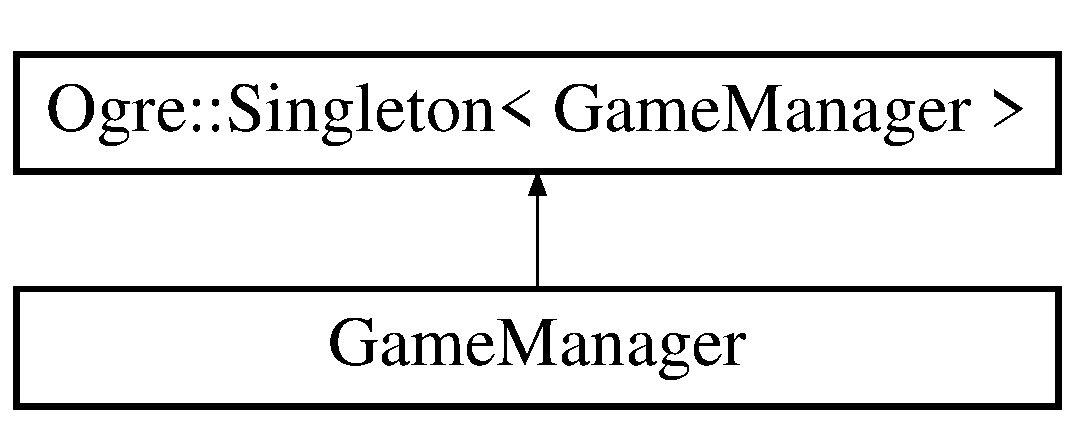
\includegraphics[height=2.000000cm]{class_game_manager}
\end{center}
\end{figure}
\subsection*{Static Public Member Functions}
\begin{DoxyCompactItemize}
\item 
\hypertarget{class_game_manager_ac55569b638688eae03c8af064a8f06af}{}static \hyperlink{class_game_manager}{Game\+Manager} \& {\bfseries Get\+Singleton} (void)\label{class_game_manager_ac55569b638688eae03c8af064a8f06af}

\item 
\hypertarget{class_game_manager_a75fe0d91afd004bbbd756a53e41add6f}{}static \hyperlink{class_game_manager}{Game\+Manager} $\ast$ {\bfseries Get\+Singleton\+Ptr} (void)\label{class_game_manager_a75fe0d91afd004bbbd756a53e41add6f}

\end{DoxyCompactItemize}
\subsection*{Public Attributes}
\begin{DoxyCompactItemize}
\item 
\hypertarget{class_game_manager_aed58f2ba9c6c6c5240095fe46698d74f}{}\hyperlink{class_input_manager}{Input\+Manager} {\bfseries m\+Input\+Manager}\label{class_game_manager_aed58f2ba9c6c6c5240095fe46698d74f}

\item 
\hypertarget{class_game_manager_a1c97a0a80e562b5c540ae63337e18810}{}Ogre\+::\+Scene\+Manager $\ast$ {\bfseries m\+Scene\+Mgr}\label{class_game_manager_a1c97a0a80e562b5c540ae63337e18810}

\item 
\hypertarget{class_game_manager_a39aace8d193db09a2137cb66b349f59b}{}Ogre\+::\+Camera $\ast$ {\bfseries m\+Camera}\label{class_game_manager_a39aace8d193db09a2137cb66b349f59b}

\item 
\hypertarget{class_game_manager_a2f1345f20f499d9ac8b1b86422922e72}{}Ogre\+::\+Render\+Window $\ast$ {\bfseries m\+Window}\label{class_game_manager_a2f1345f20f499d9ac8b1b86422922e72}

\end{DoxyCompactItemize}


The documentation for this class was generated from the following files\+:\begin{DoxyCompactItemize}
\item 
Game\+Manager.\+h\item 
Game\+Manager.\+cpp\end{DoxyCompactItemize}

\hypertarget{class_input_manager}{}\section{Input\+Manager Class Reference}
\label{class_input_manager}\index{Input\+Manager@{Input\+Manager}}
Inheritance diagram for Input\+Manager\+:\begin{figure}[H]
\begin{center}
\leavevmode
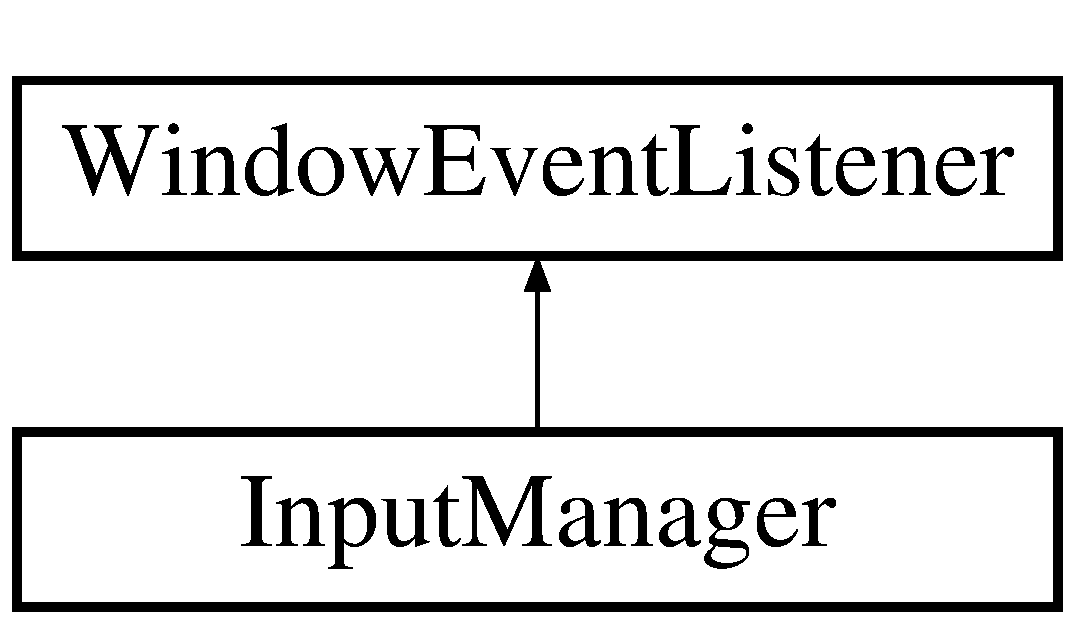
\includegraphics[height=2.000000cm]{class_input_manager}
\end{center}
\end{figure}
\subsection*{Public Member Functions}
\begin{DoxyCompactItemize}
\item 
\hypertarget{class_input_manager_a4279d1e21e43fbb588d2b02b752cf64a}{}void {\bfseries Init\+Input} (Ogre\+::\+Render\+Window $\ast$m\+Window)\label{class_input_manager_a4279d1e21e43fbb588d2b02b752cf64a}

\end{DoxyCompactItemize}
\subsection*{Public Attributes}
\begin{DoxyCompactItemize}
\item 
\hypertarget{class_input_manager_a8c44ba031e327eb7d6b58d0164381f84}{}O\+I\+S\+::\+Mouse $\ast$ {\bfseries m\+Mouse}\label{class_input_manager_a8c44ba031e327eb7d6b58d0164381f84}

\item 
\hypertarget{class_input_manager_af4b794dea8a8e3cd3edf9a1272827cf3}{}O\+I\+S\+::\+Keyboard $\ast$ {\bfseries m\+Keyboard}\label{class_input_manager_af4b794dea8a8e3cd3edf9a1272827cf3}

\end{DoxyCompactItemize}
\subsection*{Protected Member Functions}
\begin{DoxyCompactItemize}
\item 
\hypertarget{class_input_manager_a6197219d09c7d3c6d51ffbc2cb493bf1}{}virtual void {\bfseries window\+Resized} (Ogre\+::\+Render\+Window $\ast$rw)\label{class_input_manager_a6197219d09c7d3c6d51ffbc2cb493bf1}

\item 
\hypertarget{class_input_manager_aeb337d8cc54ff987cca0c73ff212d6bf}{}virtual void {\bfseries window\+Closed} (Ogre\+::\+Render\+Window $\ast$rw)\label{class_input_manager_aeb337d8cc54ff987cca0c73ff212d6bf}

\end{DoxyCompactItemize}
\subsection*{Protected Attributes}
\begin{DoxyCompactItemize}
\item 
\hypertarget{class_input_manager_aee067bb5dcb7166ed63b4e992255ccaa}{}O\+I\+S\+::\+Input\+Manager $\ast$ {\bfseries m\+Input\+Manager}\label{class_input_manager_aee067bb5dcb7166ed63b4e992255ccaa}

\end{DoxyCompactItemize}


The documentation for this class was generated from the following files\+:\begin{DoxyCompactItemize}
\item 
Input\+Manager.\+h\item 
Input\+Manager.\+cpp\end{DoxyCompactItemize}

\hypertarget{class_main}{}\section{Main Class Reference}
\label{class_main}\index{Main@{Main}}
Inheritance diagram for Main\+:\begin{figure}[H]
\begin{center}
\leavevmode
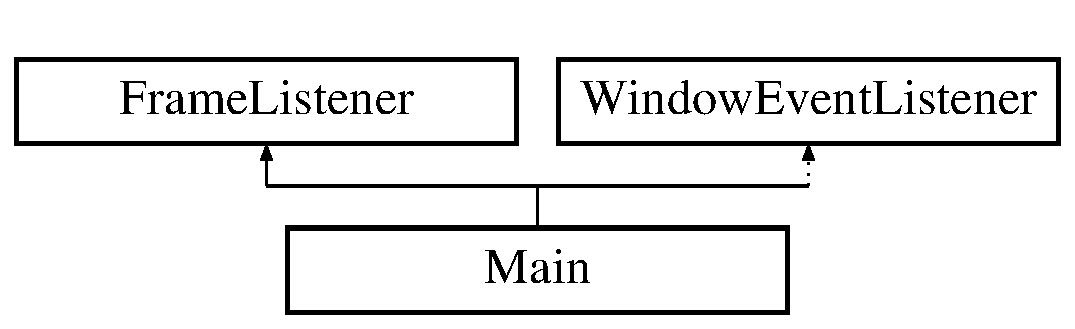
\includegraphics[height=2.000000cm]{class_main}
\end{center}
\end{figure}
\subsection*{Public Member Functions}
\begin{DoxyCompactItemize}
\item 
\hypertarget{class_main_a24eca335d9f64d276e5d42e36fbbe26e}{}bool {\bfseries go} ()\label{class_main_a24eca335d9f64d276e5d42e36fbbe26e}

\end{DoxyCompactItemize}
\subsection*{Protected Member Functions}
\begin{DoxyCompactItemize}
\item 
\hypertarget{class_main_a5f6baea1ccb9bc00f67c7e5c4a26b5af}{}virtual bool {\bfseries frame\+Rendering\+Queued} (const Ogre\+::\+Frame\+Event \&evt)\label{class_main_a5f6baea1ccb9bc00f67c7e5c4a26b5af}

\end{DoxyCompactItemize}
\subsection*{Protected Attributes}
\begin{DoxyCompactItemize}
\item 
\hypertarget{class_main_a652fc62fa43ccf55670d6c839c48743a}{}Ogre\+::\+Root $\ast$ {\bfseries m\+Root}\label{class_main_a652fc62fa43ccf55670d6c839c48743a}

\item 
\hypertarget{class_main_aff38502c06a9886eb8e671821d39f9f5}{}Ogre\+::\+String {\bfseries m\+Resources\+Cfg}\label{class_main_aff38502c06a9886eb8e671821d39f9f5}

\item 
\hypertarget{class_main_ac5974cc5633e82bc3b1e3c8341bbdab4}{}Ogre\+::\+String {\bfseries m\+Plugins\+Cfg}\label{class_main_ac5974cc5633e82bc3b1e3c8341bbdab4}

\item 
\hypertarget{class_main_ae982ce1806d05dee26bb7c89f970e21c}{}Ogre\+::\+Render\+Window $\ast$ {\bfseries m\+Window}\label{class_main_ae982ce1806d05dee26bb7c89f970e21c}

\item 
\hypertarget{class_main_a4668c9d8815ef017ae949030d870599f}{}\hyperlink{class_player}{Player} {\bfseries player}\label{class_main_a4668c9d8815ef017ae949030d870599f}

\item 
\hypertarget{class_main_af013569acae33b762f8671e7fe28e6dc}{}\hyperlink{class_main_camera}{Main\+Camera} $\ast$ {\bfseries m\+Main\+Camera}\label{class_main_af013569acae33b762f8671e7fe28e6dc}

\item 
\hypertarget{class_main_a5d46009c71d4ee9ddf0f1e4dbbdc9bfd}{}\hyperlink{class_enemy}{Enemy} {\bfseries enemy}\label{class_main_a5d46009c71d4ee9ddf0f1e4dbbdc9bfd}

\item 
\hypertarget{class_main_aabf11bb20aaced75761f6c25f7c2d240}{}Ogre\+Bites\+::\+Sdk\+Camera\+Man $\ast$ {\bfseries m\+Camera\+Man}\label{class_main_aabf11bb20aaced75761f6c25f7c2d240}

\end{DoxyCompactItemize}


The documentation for this class was generated from the following files\+:\begin{DoxyCompactItemize}
\item 
Main.\+h\item 
Main.\+cpp\end{DoxyCompactItemize}

\hypertarget{class_main_camera}{}\section{Main\+Camera Class Reference}
\label{class_main_camera}\index{Main\+Camera@{Main\+Camera}}
\subsection*{Public Member Functions}
\begin{DoxyCompactItemize}
\item 
\hypertarget{class_main_camera_a037e576d9606a1b626468959a93bb3e4}{}void {\bfseries Camera\+Instance} ()\label{class_main_camera_a037e576d9606a1b626468959a93bb3e4}

\end{DoxyCompactItemize}


The documentation for this class was generated from the following files\+:\begin{DoxyCompactItemize}
\item 
Main\+Camera.\+h\item 
Main\+Camera.\+cpp\end{DoxyCompactItemize}

\hypertarget{class_matrix4}{}\section{Matrix4 Class Reference}
\label{class_matrix4}\index{Matrix4@{Matrix4}}
\subsection*{Public Member Functions}
\begin{DoxyCompactItemize}
\item 
\hyperlink{class_matrix4_a21e70a74447b9b05cf9a06400bc9c661}{Matrix4} ()
\item 
\hyperlink{class_matrix4_a524a8a7fef110500b7e56abf03473018}{Matrix4} (const \hyperlink{class_matrix4}{Matrix4} \&rhs)
\item 
\hyperlink{class_matrix4_a378e12a6d53ad29895c9d048d7152aa9}{Matrix4} (float \+\_\+00, float \+\_\+10, float \+\_\+20, float \+\_\+30, float \+\_\+01, float \+\_\+11, float \+\_\+21, float \+\_\+31, float \+\_\+02, float \+\_\+12, float \+\_\+22, float \+\_\+32, float \+\_\+03, float \+\_\+13, float \+\_\+23, float \+\_\+33)
\item 
\hyperlink{class_matrix4_a33bdf9c4d086be1c5d6889154de9c2b4}{Matrix4} (float \&values\mbox{[}16\mbox{]})
\item 
float \& \hyperlink{class_matrix4_a3e542f89134e7496dfe820ba1668b305}{operator\mbox{[}$\,$\mbox{]}} (int index)
\item 
const float \& \hyperlink{class_matrix4_ad80f68f96c8e78ea4eed23c2745d47f2}{operator\mbox{[}$\,$\mbox{]}} (int index) const 
\item 
\hypertarget{class_matrix4_a2a7f1a5d8b2396b7ab9135ccca2b2865}{}void {\bfseries print\+Matrix4} ()\label{class_matrix4_a2a7f1a5d8b2396b7ab9135ccca2b2865}

\end{DoxyCompactItemize}
\subsection*{Static Public Member Functions}
\begin{DoxyCompactItemize}
\item 
static \hyperlink{class_matrix4}{Matrix4} \hyperlink{class_matrix4_a2a4902003a3cf712cb6baf3fb87a5c97}{Zero} ()
\item 
static \hyperlink{class_matrix4}{Matrix4} \hyperlink{class_matrix4_ae114a47efddacad2207eadac5f532098}{Identity} ()
\item 
static \hyperlink{class_matrix4}{Matrix4} \hyperlink{class_matrix4_a23836c2ff14cd2ddaca541b18a75e40b}{Transpose} (const \hyperlink{class_matrix4}{Matrix4} \&mat)
\item 
static \hyperlink{class_matrix4}{Matrix4} \hyperlink{class_matrix4_a18a798425b4832c7798faa3d9efc2353}{Set\+Translation} (const \hyperlink{class_vector3}{Vector3} \&translation)
\item 
static \hyperlink{class_vector3}{Vector3} \hyperlink{class_matrix4_a89ca1ebbb17ff31088eba0717d39081f}{Get\+Translation} (const \hyperlink{class_matrix4}{Matrix4} \&mat)
\item 
static \hyperlink{class_matrix4}{Matrix4} \hyperlink{class_matrix4_a752879f3a6c5d5d941e9ae73e765e31e}{Set\+Scale} (const \hyperlink{class_vector3}{Vector3} \&scale)
\item 
static \hyperlink{class_matrix4}{Matrix4} \hyperlink{class_matrix4_abec52734ac8ee872a518d7215a4569be}{Set\+Rotation\+Axis} (const \hyperlink{class_vector3}{Vector3} \&axis, float angle)
\item 
static \hyperlink{class_vector3}{Vector3} \hyperlink{class_matrix4_a9689e66f64c12010784feed25a85a0ca}{Transform\+Point} (const \hyperlink{class_matrix4}{Matrix4} \&mat, const \hyperlink{class_vector3}{Vector3} \&p)
\item 
static \hyperlink{class_vector3}{Vector3} \hyperlink{class_matrix4_a9fe99a8a30a59bf2ff059c3e179c8571}{Transform\+Direction} (const \hyperlink{class_matrix4}{Matrix4} \&mat, const \hyperlink{class_vector3}{Vector3} \&n)
\end{DoxyCompactItemize}
\subsection*{Public Attributes}
\begin{DoxyCompactItemize}
\item 
\hypertarget{class_matrix4_a2da02f7831b9bd25b272756d7e5eb90b}{}float {\bfseries m} \mbox{[}16\mbox{]}\label{class_matrix4_a2da02f7831b9bd25b272756d7e5eb90b}

\end{DoxyCompactItemize}


\subsection{Constructor \& Destructor Documentation}
\hypertarget{class_matrix4_a21e70a74447b9b05cf9a06400bc9c661}{}\index{Matrix4@{Matrix4}!Matrix4@{Matrix4}}
\index{Matrix4@{Matrix4}!Matrix4@{Matrix4}}
\subsubsection[{Matrix4}]{\setlength{\rightskip}{0pt plus 5cm}Matrix4\+::\+Matrix4 (
\begin{DoxyParamCaption}
{}
\end{DoxyParamCaption}
)}\label{class_matrix4_a21e70a74447b9b05cf9a06400bc9c661}
Default \hyperlink{class_matrix4}{Matrix4} constructor, creates an empty \hyperlink{class_matrix4}{Matrix4}. \hypertarget{class_matrix4_a524a8a7fef110500b7e56abf03473018}{}\index{Matrix4@{Matrix4}!Matrix4@{Matrix4}}
\index{Matrix4@{Matrix4}!Matrix4@{Matrix4}}
\subsubsection[{Matrix4}]{\setlength{\rightskip}{0pt plus 5cm}Matrix4\+::\+Matrix4 (
\begin{DoxyParamCaption}
\item[{const {\bf Matrix4} \&}]{rhs}
\end{DoxyParamCaption}
)}\label{class_matrix4_a524a8a7fef110500b7e56abf03473018}
\hyperlink{class_matrix4}{Matrix4} copy construtor, creates a \hyperlink{class_matrix4}{Matrix4} from an existing one. 
\begin{DoxyParams}{Parameters}
{\em rhs} & The \hyperlink{class_matrix4}{Matrix4} to create a copy of. \\
\hline
\end{DoxyParams}
\hypertarget{class_matrix4_a378e12a6d53ad29895c9d048d7152aa9}{}\index{Matrix4@{Matrix4}!Matrix4@{Matrix4}}
\index{Matrix4@{Matrix4}!Matrix4@{Matrix4}}
\subsubsection[{Matrix4}]{\setlength{\rightskip}{0pt plus 5cm}Matrix4\+::\+Matrix4 (
\begin{DoxyParamCaption}
\item[{float}]{\+\_\+00, }
\item[{float}]{\+\_\+10, }
\item[{float}]{\+\_\+20, }
\item[{float}]{\+\_\+30, }
\item[{float}]{\+\_\+01, }
\item[{float}]{\+\_\+11, }
\item[{float}]{\+\_\+21, }
\item[{float}]{\+\_\+31, }
\item[{float}]{\+\_\+02, }
\item[{float}]{\+\_\+12, }
\item[{float}]{\+\_\+22, }
\item[{float}]{\+\_\+32, }
\item[{float}]{\+\_\+03, }
\item[{float}]{\+\_\+13, }
\item[{float}]{\+\_\+23, }
\item[{float}]{\+\_\+33}
\end{DoxyParamCaption}
)}\label{class_matrix4_a378e12a6d53ad29895c9d048d7152aa9}
\hyperlink{class_matrix4}{Matrix4} values constructor, creates a \hyperlink{class_matrix4}{Matrix4} from 16 floats. 
\begin{DoxyParams}{Parameters}
{\em \+\_\+12} & The value in the second column and third row of the matrix. \\
\hline
\end{DoxyParams}
\hypertarget{class_matrix4_a33bdf9c4d086be1c5d6889154de9c2b4}{}\index{Matrix4@{Matrix4}!Matrix4@{Matrix4}}
\index{Matrix4@{Matrix4}!Matrix4@{Matrix4}}
\subsubsection[{Matrix4}]{\setlength{\rightskip}{0pt plus 5cm}Matrix4\+::\+Matrix4 (
\begin{DoxyParamCaption}
\item[{float \&}]{values\mbox{[}16\mbox{]}}
\end{DoxyParamCaption}
)}\label{class_matrix4_a33bdf9c4d086be1c5d6889154de9c2b4}
\hyperlink{class_matrix4}{Matrix4} array constructor, creates a 4x4 matrix from an array of 16 floats.~\newline
U\+N\+T\+E\+S\+T\+E\+D. 
\begin{DoxyParams}{Parameters}
{\em values} & The array of values to create the matrix from. \\
\hline
\end{DoxyParams}


\subsection{Member Function Documentation}
\hypertarget{class_matrix4_a89ca1ebbb17ff31088eba0717d39081f}{}\index{Matrix4@{Matrix4}!Get\+Translation@{Get\+Translation}}
\index{Get\+Translation@{Get\+Translation}!Matrix4@{Matrix4}}
\subsubsection[{Get\+Translation}]{\setlength{\rightskip}{0pt plus 5cm}{\bf Vector3} Matrix4\+::\+Get\+Translation (
\begin{DoxyParamCaption}
\item[{const {\bf Matrix4} \&}]{mat}
\end{DoxyParamCaption}
)\hspace{0.3cm}{\ttfamily [static]}}\label{class_matrix4_a89ca1ebbb17ff31088eba0717d39081f}
Get Translation method, finds the translation component of a given matrix. 
\begin{DoxyParams}{Parameters}
{\em mat} & The input matrix \\
\hline
\end{DoxyParams}
\begin{DoxyReturn}{Returns}
A \hyperlink{class_vector3}{Vector3} that is the translation component of mat. 
\end{DoxyReturn}
\hypertarget{class_matrix4_ae114a47efddacad2207eadac5f532098}{}\index{Matrix4@{Matrix4}!Identity@{Identity}}
\index{Identity@{Identity}!Matrix4@{Matrix4}}
\subsubsection[{Identity}]{\setlength{\rightskip}{0pt plus 5cm}{\bf Matrix4} Matrix4\+::\+Identity (
\begin{DoxyParamCaption}
{}
\end{DoxyParamCaption}
)\hspace{0.3cm}{\ttfamily [static]}}\label{class_matrix4_ae114a47efddacad2207eadac5f532098}
Identity method, creates an identity matrix. \begin{DoxyReturn}{Returns}
A matrix whose values are 1 on the leading diagonal and 0 everywhere else. 
\end{DoxyReturn}
\hypertarget{class_matrix4_a3e542f89134e7496dfe820ba1668b305}{}\index{Matrix4@{Matrix4}!operator\mbox{[}$\,$\mbox{]}@{operator[]}}
\index{operator\mbox{[}$\,$\mbox{]}@{operator[]}!Matrix4@{Matrix4}}
\subsubsection[{operator[]}]{\setlength{\rightskip}{0pt plus 5cm}float \& Matrix4\+::operator\mbox{[}$\,$\mbox{]} (
\begin{DoxyParamCaption}
\item[{int}]{index}
\end{DoxyParamCaption}
)}\label{class_matrix4_a3e542f89134e7496dfe820ba1668b305}
\mbox{[}\mbox{]} operator, returns the value of a float at an index. 
\begin{DoxyParams}{Parameters}
{\em index} & The index at which the value lies. \\
\hline
\end{DoxyParams}
\begin{DoxyReturn}{Returns}
The value at that index. 
\end{DoxyReturn}
\hypertarget{class_matrix4_ad80f68f96c8e78ea4eed23c2745d47f2}{}\index{Matrix4@{Matrix4}!operator\mbox{[}$\,$\mbox{]}@{operator[]}}
\index{operator\mbox{[}$\,$\mbox{]}@{operator[]}!Matrix4@{Matrix4}}
\subsubsection[{operator[]}]{\setlength{\rightskip}{0pt plus 5cm}const float \& Matrix4\+::operator\mbox{[}$\,$\mbox{]} (
\begin{DoxyParamCaption}
\item[{int}]{index}
\end{DoxyParamCaption}
) const}\label{class_matrix4_ad80f68f96c8e78ea4eed23c2745d47f2}
Static \mbox{[}\mbox{]} operator, retrieves the value of a float at an index and does not modify it. 
\begin{DoxyParams}{Parameters}
{\em index} & The index at which the value lies. \\
\hline
\end{DoxyParams}
\begin{DoxyReturn}{Returns}
The value at that index. 
\end{DoxyReturn}
\hypertarget{class_matrix4_abec52734ac8ee872a518d7215a4569be}{}\index{Matrix4@{Matrix4}!Set\+Rotation\+Axis@{Set\+Rotation\+Axis}}
\index{Set\+Rotation\+Axis@{Set\+Rotation\+Axis}!Matrix4@{Matrix4}}
\subsubsection[{Set\+Rotation\+Axis}]{\setlength{\rightskip}{0pt plus 5cm}{\bf Matrix4} Matrix4\+::\+Set\+Rotation\+Axis (
\begin{DoxyParamCaption}
\item[{const {\bf Vector3} \&}]{axis, }
\item[{float}]{angle}
\end{DoxyParamCaption}
)\hspace{0.3cm}{\ttfamily [static]}}\label{class_matrix4_abec52734ac8ee872a518d7215a4569be}
Set Rotation Axis, sets up a rotation matrix about a vector by an angle. 
\begin{DoxyParams}{Parameters}
{\em axis} & A \hyperlink{class_vector3}{Vector3} representing an axis to rotate around. \\
\hline
{\em angle} & An angle in radians to rotate by. \\
\hline
\end{DoxyParams}
\hypertarget{class_matrix4_a752879f3a6c5d5d941e9ae73e765e31e}{}\index{Matrix4@{Matrix4}!Set\+Scale@{Set\+Scale}}
\index{Set\+Scale@{Set\+Scale}!Matrix4@{Matrix4}}
\subsubsection[{Set\+Scale}]{\setlength{\rightskip}{0pt plus 5cm}{\bf Matrix4} Matrix4\+::\+Set\+Scale (
\begin{DoxyParamCaption}
\item[{const {\bf Vector3} \&}]{scale}
\end{DoxyParamCaption}
)\hspace{0.3cm}{\ttfamily [static]}}\label{class_matrix4_a752879f3a6c5d5d941e9ae73e765e31e}
Scale operation, creates an identity matrix with scale components set by an input vector.~\newline
Scales in x, y and z. 
\begin{DoxyParams}{Parameters}
{\em scale} & A \hyperlink{class_vector3}{Vector3} containing the scale . \\
\hline
\end{DoxyParams}
\begin{DoxyReturn}{Returns}
An identity \hyperlink{class_matrix4}{Matrix4} whose scale components are defined by the input vector. 
\end{DoxyReturn}
\hypertarget{class_matrix4_a18a798425b4832c7798faa3d9efc2353}{}\index{Matrix4@{Matrix4}!Set\+Translation@{Set\+Translation}}
\index{Set\+Translation@{Set\+Translation}!Matrix4@{Matrix4}}
\subsubsection[{Set\+Translation}]{\setlength{\rightskip}{0pt plus 5cm}{\bf Matrix4} Matrix4\+::\+Set\+Translation (
\begin{DoxyParamCaption}
\item[{const {\bf Vector3} \&}]{translation}
\end{DoxyParamCaption}
)\hspace{0.3cm}{\ttfamily [static]}}\label{class_matrix4_a18a798425b4832c7798faa3d9efc2353}
Set Translation method, sets the values of the matrix that would modify the position when applied to a vector. 
\begin{DoxyParams}{Parameters}
{\em translation} & A translation vector. \\
\hline
\end{DoxyParams}
\begin{DoxyReturn}{Returns}
An identity matrix whose translation values are modified by the input vector. 
\end{DoxyReturn}
\hypertarget{class_matrix4_a9fe99a8a30a59bf2ff059c3e179c8571}{}\index{Matrix4@{Matrix4}!Transform\+Direction@{Transform\+Direction}}
\index{Transform\+Direction@{Transform\+Direction}!Matrix4@{Matrix4}}
\subsubsection[{Transform\+Direction}]{\setlength{\rightskip}{0pt plus 5cm}{\bf Vector3} Matrix4\+::\+Transform\+Direction (
\begin{DoxyParamCaption}
\item[{const {\bf Matrix4} \&}]{mat, }
\item[{const {\bf Vector3} \&}]{n}
\end{DoxyParamCaption}
)\hspace{0.3cm}{\ttfamily [static]}}\label{class_matrix4_a9fe99a8a30a59bf2ff059c3e179c8571}
Method to transform a direction vector by a given matrix.~\newline
Note that matrix multiplication is non-\/commutative. 
\begin{DoxyParams}{Parameters}
{\em mat} & A transformation matrix. \\
\hline
{\em n} & A normalized direction vector to transform. \\
\hline
\end{DoxyParams}
\begin{DoxyReturn}{Returns}
The transformed direction vector. 
\end{DoxyReturn}
\hypertarget{class_matrix4_a9689e66f64c12010784feed25a85a0ca}{}\index{Matrix4@{Matrix4}!Transform\+Point@{Transform\+Point}}
\index{Transform\+Point@{Transform\+Point}!Matrix4@{Matrix4}}
\subsubsection[{Transform\+Point}]{\setlength{\rightskip}{0pt plus 5cm}{\bf Vector3} Matrix4\+::\+Transform\+Point (
\begin{DoxyParamCaption}
\item[{const {\bf Matrix4} \&}]{mat, }
\item[{const {\bf Vector3} \&}]{p}
\end{DoxyParamCaption}
)\hspace{0.3cm}{\ttfamily [static]}}\label{class_matrix4_a9689e66f64c12010784feed25a85a0ca}
Method to transform a point vector by a given matrix.~\newline
p and m are not modified. 
\begin{DoxyParams}{Parameters}
{\em mat} & The transformation matrix. \\
\hline
{\em p} & The point vector that will be transformed. \\
\hline
\end{DoxyParams}
\begin{DoxyReturn}{Returns}
A \hyperlink{class_vector3}{Vector3} that is p transformed by m. 
\end{DoxyReturn}
\hypertarget{class_matrix4_a23836c2ff14cd2ddaca541b18a75e40b}{}\index{Matrix4@{Matrix4}!Transpose@{Transpose}}
\index{Transpose@{Transpose}!Matrix4@{Matrix4}}
\subsubsection[{Transpose}]{\setlength{\rightskip}{0pt plus 5cm}{\bf Matrix4} Matrix4\+::\+Transpose (
\begin{DoxyParamCaption}
\item[{const {\bf Matrix4} \&}]{mat}
\end{DoxyParamCaption}
)\hspace{0.3cm}{\ttfamily [static]}}\label{class_matrix4_a23836c2ff14cd2ddaca541b18a75e40b}
Transpose method, swaps the rows and columns of a matrix. 
\begin{DoxyParams}{Parameters}
{\em mat} & The matrix to be transposed. \\
\hline
\end{DoxyParams}
\begin{DoxyReturn}{Returns}
A transposed version of the input matrix. 
\end{DoxyReturn}
\hypertarget{class_matrix4_a2a4902003a3cf712cb6baf3fb87a5c97}{}\index{Matrix4@{Matrix4}!Zero@{Zero}}
\index{Zero@{Zero}!Matrix4@{Matrix4}}
\subsubsection[{Zero}]{\setlength{\rightskip}{0pt plus 5cm}{\bf Matrix4} Matrix4\+::\+Zero (
\begin{DoxyParamCaption}
{}
\end{DoxyParamCaption}
)\hspace{0.3cm}{\ttfamily [static]}}\label{class_matrix4_a2a4902003a3cf712cb6baf3fb87a5c97}
Zero method, returns a zero-\/matrix. \begin{DoxyReturn}{Returns}
An empty matrix (a matrix filled with zeros). 
\end{DoxyReturn}


The documentation for this class was generated from the following files\+:\begin{DoxyCompactItemize}
\item 
Matrix4.\+h\item 
Matrix4.\+cpp\end{DoxyCompactItemize}

\hypertarget{class_matth}{}\section{Matth Class Reference}
\label{class_matth}\index{Matth@{Matth}}
\subsection*{Static Public Member Functions}
\begin{DoxyCompactItemize}
\item 
static int \hyperlink{class_matth_a900bf48507faeeb54a59213b62c00214}{absi} (const int value)
\item 
static float \hyperlink{class_matth_abfedd79c6ae1ce550784f17bf406da16}{abs} (const float value)
\item 
static float \hyperlink{class_matth_a6434126a05ec38e24a128bbc4e8938c4}{acos} (const float value)
\item 
static float \hyperlink{class_matth_a968adf68a678d9c56665dbabf246a6d4}{asin} (const float value)
\item 
static float \hyperlink{class_matth_a432ca1cc25b6e072129fbeb1a114b9f7}{atan} (const float value)
\item 
static float \hyperlink{class_matth_a5846ab2422a3d4f5968d5e0a8e135d0e}{atan2} (const float x, const float y)
\item 
static bool \hyperlink{class_matth_ad575860c76bd54d7ff8b8b889083a4d5}{approximately} (const float x, const float y)
\item 
static float \hyperlink{class_matth_a5cd315282b3dab72af5eaab3b5ade677}{average} (const float x, const float y)
\item 
static float \hyperlink{class_matth_a24f54a878a9c245b07293bcb942d76b4}{average} (const int x, const float y)
\item 
static float \hyperlink{class_matth_a7889849995bd56e78825a685fa3cf296}{average} (const int x, const int y)
\item 
static int \hyperlink{class_matth_a3b290e67eb4d4dcb2407edbeeed7822d}{ceili} (const float value)
\item 
static float \hyperlink{class_matth_a0f6e05dbb4d1b776420bc4a8c66e8eb4}{ceil} (const float value)
\item 
static int \hyperlink{class_matth_a81a58aa02e55ace490ff154b85a3c57e}{clampi} (const int value, const int min, const int max)
\item 
static float \hyperlink{class_matth_a5da791959fa3f433ae1746f3d6d5e592}{clamp} (const float value, const float min, const float max)
\item 
static float \hyperlink{class_matth_afe555e1bdec52d87807b172d1aa132d9}{clamp01} (const float value)
\item 
\hypertarget{class_matth_a9cb31c1d7333f316d5914ebfafc676de}{}static int {\bfseries closest\+Power\+Of\+Two} (const float value)\label{class_matth_a9cb31c1d7333f316d5914ebfafc676de}

\item 
\hypertarget{class_matth_a620766386242a964ad4c776f1209839f}{}static int {\bfseries closest\+Power\+Of\+Two} (const int value)\label{class_matth_a620766386242a964ad4c776f1209839f}

\item 
static float \hyperlink{class_matth_ab36b9435c9beb3f760d85b384826a032}{cos} (const float value)
\item 
static float \hyperlink{class_matth_afa0d084b15462e8c7e54b1bf4b0af288}{sin} (const float value)
\item 
static float \hyperlink{class_matth_ad09a3b61cc9e6a97f58bc6371f18e2ac}{tan} (const float value)
\item 
static float \hyperlink{class_matth_a94a0265fe56178120283cc50244ac8a9}{cot} (const float value)
\item 
static float \hyperlink{class_matth_a5224f6cd5d3920845d41942471b360a5}{sec} (const float value)
\item 
static float \hyperlink{class_matth_a33e26fbbf97fe67c24a7c14196b17c01}{csc} (const float value)
\item 
\hypertarget{class_matth_a3a3575a3f3db638f7e68bbbee42968ee}{}static float {\bfseries delta\+Angle} (const float current, const float target)\label{class_matth_a3a3575a3f3db638f7e68bbbee42968ee}

\item 
static float \hyperlink{class_matth_a75024342e85cc72f80c45d5a8f3564f1}{exp} (const float power)
\item 
static float \hyperlink{class_matth_ac4514a2a57c120f5b51719c7d95b3e8b}{exps} (const int power)
\item 
static int \hyperlink{class_matth_a7431c576ec39c974f575f040833f9d95}{floori} (const float value)
\item 
static float \hyperlink{class_matth_af380b2262ba103544e70d752287390e2}{floor} (const float value)
\item 
static float \hyperlink{class_matth_af61c67de0420e844f576b2b29c9daaef}{linear\+To\+Gamma\+Space} (const float value)
\item 
static float \hyperlink{class_matth_a94df1fe53e38f3200cb53a044ca82eb7}{gamma\+To\+Linear\+Space} (const float value)
\item 
static bool \hyperlink{class_matth_a0347598feecff1d5851f33324034f98c}{is\+Power\+Of\+Two} (const int value)
\item 
static bool \hyperlink{class_matth_a16bde0574496581105e37db358e81bf1}{is\+Power\+Of\+Twoe} (const int value)
\item 
static float \hyperlink{class_matth_a656a8b2b10a5270f247bb26d7f709537}{lerp} (const float start, const float end, const float value)
\item 
\hypertarget{class_matth_a6c969a645eb5824d6e698bce205460cd}{}static float {\bfseries lerp\+Angle} (const float start, const float end, const float value)\label{class_matth_a6c969a645eb5824d6e698bce205460cd}

\item 
static float \hyperlink{class_matth_a6336a42efd5500e7c470a04eefbcb778}{lerp\+Unclamped} (const float start, const float end, const float value)
\item 
static float \hyperlink{class_matth_a0f4cf803a6e526cd3917810a5f151886}{inverse\+Lerp} (const float start, const float end, const float value)
\item 
static float \hyperlink{class_matth_afba8bc869a1847fa5ea6f2d7ddd66df8}{log} (const int value, const int base=10)
\item 
static float \hyperlink{class_matth_aeee95b77e08d2b8eeb765cba3d3428ef}{log} (const int value, const float base=10.\+0f)
\item 
static float \hyperlink{class_matth_a3b3c174cf818dafa2bb0868c0be2d91a}{log} (const float value, const float base=10.\+0f)
\item 
static float \hyperlink{class_matth_a63ba77faee2dc493e1c23592139426af}{ln} (const int value)
\item 
static float \hyperlink{class_matth_a2e6c35db4051df0578fab51d4ae794b9}{ln} (const float value, int prec=3)
\item 
static bool \hyperlink{class_matth_ac159082536b46168144c41a4d60e2b83}{logical\+X\+O\+R} (const bool a, const bool b)
\item 
\hypertarget{class_matth_a4f366db2949ecfe682dab88bdcf3a824}{}static float {\bfseries move\+Towards} (const float current, const float target, const float max\+Delta)\label{class_matth_a4f366db2949ecfe682dab88bdcf3a824}

\item 
\hypertarget{class_matth_a4e035c33e43aa8bef4c9b548397732e6}{}static float {\bfseries move\+Towards\+Angle} (const float current, const float target, const float max\+Delta)\label{class_matth_a4e035c33e43aa8bef4c9b548397732e6}

\item 
static int \hyperlink{class_matth_a14ad60da4d1beb165d75ee063507d5f5}{next\+Power\+Of\+Two} (const int value)
\item 
static int \hyperlink{class_matth_ab5995f6ad58e9f09fdc30e7978276e68}{next\+Power\+Of\+Two} (const float value)
\item 
static int \hyperlink{class_matth_a930836f29bc1538f8089ccf70a511792}{next\+Power\+Of\+Twoe} (const float value)
\item 
\hypertarget{class_matth_a08350dffcf04a66a87cbf81897f1f148}{}static float {\bfseries perlin\+Noise} (const float x, const float y)\label{class_matth_a08350dffcf04a66a87cbf81897f1f148}

\item 
\hypertarget{class_matth_a04ea1eb756abb1fa8bdec988e683dece}{}static float {\bfseries ping\+Pong} (const float value, const float length)\label{class_matth_a04ea1eb756abb1fa8bdec988e683dece}

\item 
static int \hyperlink{class_matth_af03a50b476584039c3cc3a0d0e3e9bd3}{powi} (const int x, const int y)
\item 
static float \hyperlink{class_matth_a7954d1a0bb6c622a6f549c32d2433033}{powm} (int x, int y)
\item 
static float \hyperlink{class_matth_ac278215a09c78414ba39aa272467daaa}{pow} (const float x, const int y)
\item 
static float \hyperlink{class_matth_a380eeb8581001889bdfe4ee92c37078a}{powf} (const float x, const float y)
\item 
static float \hyperlink{class_matth_a5e08b96ca233f47eb8d032f5047699e6}{pows} (const float x, const float y)
\item 
\hypertarget{class_matth_ab23724db6cbd9e4a87810de3a9b0b257}{}static float {\bfseries repeat} (const float value, const float length)\label{class_matth_ab23724db6cbd9e4a87810de3a9b0b257}

\item 
static int \hyperlink{class_matth_a7b01f3385d703849bb2fa5455240ee72}{roundi} (const float value)
\item 
static float \hyperlink{class_matth_a087cbb3b6860ceb84cb18229f8e650e8}{round} (const float value)
\item 
static int \hyperlink{class_matth_ae80bf23688c9ab836d0efe34353015b8}{sign} (const int value)
\item 
static int \hyperlink{class_matth_ac023116fb53d5ae66dd98c267ffafcf2}{sign} (const float value)
\item 
static bool \hyperlink{class_matth_adc580377dc220725fca144b52658e90b}{is\+Positive} (const int value)
\item 
static bool \hyperlink{class_matth_a4bcb12e944d790f1e5279a2a67216b9c}{is\+Positive} (const float value)
\item 
static bool \hyperlink{class_matth_a0b74da83e267dd3dabab08c698d945b9}{is\+Negative} (const int value)
\item 
static bool \hyperlink{class_matth_abcf0f572e8d5b6ff2e7dcacb7b45f171}{is\+Negative} (const float value)
\item 
static int \hyperlink{class_matth_ab274e2dde5096d43ab5255c74bf4cab1}{sqrti} (const int value)
\item 
static float \hyperlink{class_matth_a79c7e3aac560ddf3bdc454e2dd00997d}{sqrt} (const int value)
\item 
static float \hyperlink{class_matth_aa44ccf6d43d7b3e7e37988b87fd29d23}{sqrt} (const float value, int prec=8)
\item 
static float \hyperlink{class_matth_a4ee96c6fa0a8a7e0ed3ea73219104418}{F\+I\+I\+S\+R\+B\+O\+Q3\+C} (const float value)
\item 
static float \hyperlink{class_matth_acea19471a1994e0012ef8b67d450cd65}{sqrt\+With\+Natural\+Log} (const float value)
\end{DoxyCompactItemize}


\subsection{Member Function Documentation}
\hypertarget{class_matth_abfedd79c6ae1ce550784f17bf406da16}{}\index{Matth@{Matth}!abs@{abs}}
\index{abs@{abs}!Matth@{Matth}}
\subsubsection[{abs}]{\setlength{\rightskip}{0pt plus 5cm}float Matth\+::abs (
\begin{DoxyParamCaption}
\item[{const float}]{value}
\end{DoxyParamCaption}
)\hspace{0.3cm}{\ttfamily [static]}}\label{class_matth_abfedd79c6ae1ce550784f17bf406da16}
Absolute function, returns the floating point value of the input. 
\begin{DoxyParams}{Parameters}
{\em value} & The input parameter, a positive or negative float. \\
\hline
\end{DoxyParams}
\begin{DoxyReturn}{Returns}
The positive version of the input parameter. 
\end{DoxyReturn}
\hypertarget{class_matth_a900bf48507faeeb54a59213b62c00214}{}\index{Matth@{Matth}!absi@{absi}}
\index{absi@{absi}!Matth@{Matth}}
\subsubsection[{absi}]{\setlength{\rightskip}{0pt plus 5cm}int Matth\+::absi (
\begin{DoxyParamCaption}
\item[{const int}]{value}
\end{DoxyParamCaption}
)\hspace{0.3cm}{\ttfamily [static]}}\label{class_matth_a900bf48507faeeb54a59213b62c00214}
Absolute Integer function, returns the absolute value of an integer. 
\begin{DoxyParams}{Parameters}
{\em value} & The input parameter, a positive or negative integer. \\
\hline
\end{DoxyParams}
\begin{DoxyReturn}{Returns}
The positive integral version of the input. 
\end{DoxyReturn}
\hypertarget{class_matth_a6434126a05ec38e24a128bbc4e8938c4}{}\index{Matth@{Matth}!acos@{acos}}
\index{acos@{acos}!Matth@{Matth}}
\subsubsection[{acos}]{\setlength{\rightskip}{0pt plus 5cm}float Matth\+::acos (
\begin{DoxyParamCaption}
\item[{const float}]{value}
\end{DoxyParamCaption}
)\hspace{0.3cm}{\ttfamily [static]}}\label{class_matth_a6434126a05ec38e24a128bbc4e8938c4}
Inverse cosine function, returns the inverse cosine of the input in radians. 
\begin{DoxyParams}{Parameters}
{\em value} & The angle, in radians, to perform the operation on. \\
\hline
\end{DoxyParams}
\begin{DoxyReturn}{Returns}
The floating point value of the inverse cosine of the input. 
\end{DoxyReturn}
\hypertarget{class_matth_ad575860c76bd54d7ff8b8b889083a4d5}{}\index{Matth@{Matth}!approximately@{approximately}}
\index{approximately@{approximately}!Matth@{Matth}}
\subsubsection[{approximately}]{\setlength{\rightskip}{0pt plus 5cm}bool Matth\+::approximately (
\begin{DoxyParamCaption}
\item[{const float}]{x, }
\item[{const float}]{y}
\end{DoxyParamCaption}
)\hspace{0.3cm}{\ttfamily [static]}}\label{class_matth_ad575860c76bd54d7ff8b8b889083a4d5}
Approximately function, returns true if the two values are approximately equal. 
\begin{DoxyParams}{Parameters}
{\em x} & The first value. \\
\hline
{\em y} & The second value. \\
\hline
\end{DoxyParams}
\begin{DoxyReturn}{Returns}
A boolean that is true if both values are equal when rounded. 
\end{DoxyReturn}
\hypertarget{class_matth_a968adf68a678d9c56665dbabf246a6d4}{}\index{Matth@{Matth}!asin@{asin}}
\index{asin@{asin}!Matth@{Matth}}
\subsubsection[{asin}]{\setlength{\rightskip}{0pt plus 5cm}float Matth\+::asin (
\begin{DoxyParamCaption}
\item[{const float}]{value}
\end{DoxyParamCaption}
)\hspace{0.3cm}{\ttfamily [static]}}\label{class_matth_a968adf68a678d9c56665dbabf246a6d4}
Inverse sine function, returns the inverse sine of the input in radians. 
\begin{DoxyParams}{Parameters}
{\em value} & The angle, in radians, to perform the operation on. \\
\hline
\end{DoxyParams}
\begin{DoxyReturn}{Returns}
The floating point value of the inverse sine of the input. 
\end{DoxyReturn}
\hypertarget{class_matth_a432ca1cc25b6e072129fbeb1a114b9f7}{}\index{Matth@{Matth}!atan@{atan}}
\index{atan@{atan}!Matth@{Matth}}
\subsubsection[{atan}]{\setlength{\rightskip}{0pt plus 5cm}float Matth\+::atan (
\begin{DoxyParamCaption}
\item[{const float}]{value}
\end{DoxyParamCaption}
)\hspace{0.3cm}{\ttfamily [static]}}\label{class_matth_a432ca1cc25b6e072129fbeb1a114b9f7}
Inverse tangent function, returns the inverse tangent of the input in radians. 
\begin{DoxyParams}{Parameters}
{\em value} & The angle, in radians, to perform the operation on. \\
\hline
\end{DoxyParams}
\begin{DoxyReturn}{Returns}
The floating point value of the inverse tangent of the input. 
\end{DoxyReturn}
\hypertarget{class_matth_a5846ab2422a3d4f5968d5e0a8e135d0e}{}\index{Matth@{Matth}!atan2@{atan2}}
\index{atan2@{atan2}!Matth@{Matth}}
\subsubsection[{atan2}]{\setlength{\rightskip}{0pt plus 5cm}float Matth\+::atan2 (
\begin{DoxyParamCaption}
\item[{const float}]{y, }
\item[{const float}]{x}
\end{DoxyParamCaption}
)\hspace{0.3cm}{\ttfamily [static]}}\label{class_matth_a5846ab2422a3d4f5968d5e0a8e135d0e}
The two-\/parameter version of the arctangent function. Will not divide by 0. Returns 0 when the result would be infinite. 
\begin{DoxyParams}{Parameters}
{\em y} & The y coordinate \\
\hline
{\em x} & The x coordinate \\
\hline
\end{DoxyParams}
\begin{DoxyReturn}{Returns}
The angle in radians between the positive x-\/axis and the point (x, y) 
\end{DoxyReturn}
\hypertarget{class_matth_a5cd315282b3dab72af5eaab3b5ade677}{}\index{Matth@{Matth}!average@{average}}
\index{average@{average}!Matth@{Matth}}
\subsubsection[{average}]{\setlength{\rightskip}{0pt plus 5cm}float Matth\+::average (
\begin{DoxyParamCaption}
\item[{const float}]{x, }
\item[{const float}]{y}
\end{DoxyParamCaption}
)\hspace{0.3cm}{\ttfamily [static]}}\label{class_matth_a5cd315282b3dab72af5eaab3b5ade677}
Average function, finds the average between two values. 
\begin{DoxyParams}{Parameters}
{\em x} & The first value. \\
\hline
{\em y} & The second value. \\
\hline
\end{DoxyParams}
\begin{DoxyReturn}{Returns}
The mean value of x and y. 
\end{DoxyReturn}
\hypertarget{class_matth_a24f54a878a9c245b07293bcb942d76b4}{}\index{Matth@{Matth}!average@{average}}
\index{average@{average}!Matth@{Matth}}
\subsubsection[{average}]{\setlength{\rightskip}{0pt plus 5cm}float Matth\+::average (
\begin{DoxyParamCaption}
\item[{const int}]{x, }
\item[{const float}]{y}
\end{DoxyParamCaption}
)\hspace{0.3cm}{\ttfamily [static]}}\label{class_matth_a24f54a878a9c245b07293bcb942d76b4}
Average function, finds the average between an int and a float. 
\begin{DoxyParams}{Parameters}
{\em x} & The first value. \\
\hline
{\em y} & The second value. \\
\hline
\end{DoxyParams}
\begin{DoxyReturn}{Returns}
The mean value of x and y. 
\end{DoxyReturn}
\hypertarget{class_matth_a7889849995bd56e78825a685fa3cf296}{}\index{Matth@{Matth}!average@{average}}
\index{average@{average}!Matth@{Matth}}
\subsubsection[{average}]{\setlength{\rightskip}{0pt plus 5cm}float Matth\+::average (
\begin{DoxyParamCaption}
\item[{const int}]{x, }
\item[{const int}]{y}
\end{DoxyParamCaption}
)\hspace{0.3cm}{\ttfamily [static]}}\label{class_matth_a7889849995bd56e78825a685fa3cf296}
Average function, finds the average between two integers. 
\begin{DoxyParams}{Parameters}
{\em x} & The first value. \\
\hline
{\em y} & The second value. \\
\hline
\end{DoxyParams}
\begin{DoxyReturn}{Returns}
The mean value of x and y. 
\end{DoxyReturn}
\hypertarget{class_matth_a0f6e05dbb4d1b776420bc4a8c66e8eb4}{}\index{Matth@{Matth}!ceil@{ceil}}
\index{ceil@{ceil}!Matth@{Matth}}
\subsubsection[{ceil}]{\setlength{\rightskip}{0pt plus 5cm}float Matth\+::ceil (
\begin{DoxyParamCaption}
\item[{const float}]{value}
\end{DoxyParamCaption}
)\hspace{0.3cm}{\ttfamily [static]}}\label{class_matth_a0f6e05dbb4d1b776420bc4a8c66e8eb4}
Ceiling function, returns a float of the input rounded up. 
\begin{DoxyParams}{Parameters}
{\em value} & The input value. \\
\hline
\end{DoxyParams}
\begin{DoxyReturn}{Returns}
The rounded up version of the input as a float. 
\end{DoxyReturn}
\hypertarget{class_matth_a3b290e67eb4d4dcb2407edbeeed7822d}{}\index{Matth@{Matth}!ceili@{ceili}}
\index{ceili@{ceili}!Matth@{Matth}}
\subsubsection[{ceili}]{\setlength{\rightskip}{0pt plus 5cm}int Matth\+::ceili (
\begin{DoxyParamCaption}
\item[{const float}]{value}
\end{DoxyParamCaption}
)\hspace{0.3cm}{\ttfamily [static]}}\label{class_matth_a3b290e67eb4d4dcb2407edbeeed7822d}
Ceiling function, returns an integer of the input rounded up. 
\begin{DoxyParams}{Parameters}
{\em value} & The input value. \\
\hline
\end{DoxyParams}
\begin{DoxyReturn}{Returns}
The rounded up version of the input as an int. 
\end{DoxyReturn}
\hypertarget{class_matth_a5da791959fa3f433ae1746f3d6d5e592}{}\index{Matth@{Matth}!clamp@{clamp}}
\index{clamp@{clamp}!Matth@{Matth}}
\subsubsection[{clamp}]{\setlength{\rightskip}{0pt plus 5cm}float Matth\+::clamp (
\begin{DoxyParamCaption}
\item[{const float}]{value, }
\item[{const float}]{min, }
\item[{const float}]{max}
\end{DoxyParamCaption}
)\hspace{0.3cm}{\ttfamily [static]}}\label{class_matth_a5da791959fa3f433ae1746f3d6d5e592}
Clamping function, returns the clamped value of the input between a specified maximum and a specified minimum. 
\begin{DoxyParams}{Parameters}
{\em value} & The input value. \\
\hline
{\em min} & The minimum value. \\
\hline
{\em max} & The maximum value. \\
\hline
\end{DoxyParams}
\begin{DoxyReturn}{Returns}
The clamped version of the input between min and max as a float. 
\end{DoxyReturn}
\hypertarget{class_matth_afe555e1bdec52d87807b172d1aa132d9}{}\index{Matth@{Matth}!clamp01@{clamp01}}
\index{clamp01@{clamp01}!Matth@{Matth}}
\subsubsection[{clamp01}]{\setlength{\rightskip}{0pt plus 5cm}float Matth\+::clamp01 (
\begin{DoxyParamCaption}
\item[{const float}]{value}
\end{DoxyParamCaption}
)\hspace{0.3cm}{\ttfamily [static]}}\label{class_matth_afe555e1bdec52d87807b172d1aa132d9}
Clamping function, returns a floating point number clamped between 0 and 1. 
\begin{DoxyParams}{Parameters}
{\em value} & The value to be clamped. \\
\hline
\end{DoxyParams}
\begin{DoxyReturn}{Returns}
The clamped value. 
\end{DoxyReturn}
\hypertarget{class_matth_a81a58aa02e55ace490ff154b85a3c57e}{}\index{Matth@{Matth}!clampi@{clampi}}
\index{clampi@{clampi}!Matth@{Matth}}
\subsubsection[{clampi}]{\setlength{\rightskip}{0pt plus 5cm}int Matth\+::clampi (
\begin{DoxyParamCaption}
\item[{const int}]{value, }
\item[{const int}]{min, }
\item[{const int}]{max}
\end{DoxyParamCaption}
)\hspace{0.3cm}{\ttfamily [static]}}\label{class_matth_a81a58aa02e55ace490ff154b85a3c57e}
Clamping function, returns the clamped value of the input between a specified maximum and a specified minimum. 
\begin{DoxyParams}{Parameters}
{\em value} & The input value. \\
\hline
{\em min} & The minimum value. \\
\hline
{\em max} & The maximum value. \\
\hline
\end{DoxyParams}
\begin{DoxyReturn}{Returns}
The clamped version of the input between min and max as an integer. 
\end{DoxyReturn}
\hypertarget{class_matth_ab36b9435c9beb3f760d85b384826a032}{}\index{Matth@{Matth}!cos@{cos}}
\index{cos@{cos}!Matth@{Matth}}
\subsubsection[{cos}]{\setlength{\rightskip}{0pt plus 5cm}float Matth\+::cos (
\begin{DoxyParamCaption}
\item[{const float}]{value}
\end{DoxyParamCaption}
)\hspace{0.3cm}{\ttfamily [static]}}\label{class_matth_ab36b9435c9beb3f760d85b384826a032}
Cosine function, returns the cosine of the input in radians. 
\begin{DoxyParams}{Parameters}
{\em value} & The angle in radians to be cosined. \\
\hline
\end{DoxyParams}
\begin{DoxyReturn}{Returns}
The cosined value. 
\end{DoxyReturn}
\hypertarget{class_matth_a94a0265fe56178120283cc50244ac8a9}{}\index{Matth@{Matth}!cot@{cot}}
\index{cot@{cot}!Matth@{Matth}}
\subsubsection[{cot}]{\setlength{\rightskip}{0pt plus 5cm}float Matth\+::cot (
\begin{DoxyParamCaption}
\item[{const float}]{value}
\end{DoxyParamCaption}
)\hspace{0.3cm}{\ttfamily [static]}}\label{class_matth_a94a0265fe56178120283cc50244ac8a9}
Cotangent function, returns the ratio of the adjacent side of the input angle in radians to the opposite side. (Of a right-\/angled triangle) 
\begin{DoxyParams}{Parameters}
{\em value} & The angle in radians to be used in the operation. \\
\hline
\end{DoxyParams}
\begin{DoxyReturn}{Returns}
The result of the cotangent operation on the input. 
\end{DoxyReturn}
\hypertarget{class_matth_a33e26fbbf97fe67c24a7c14196b17c01}{}\index{Matth@{Matth}!csc@{csc}}
\index{csc@{csc}!Matth@{Matth}}
\subsubsection[{csc}]{\setlength{\rightskip}{0pt plus 5cm}float Matth\+::csc (
\begin{DoxyParamCaption}
\item[{const float}]{value}
\end{DoxyParamCaption}
)\hspace{0.3cm}{\ttfamily [static]}}\label{class_matth_a33e26fbbf97fe67c24a7c14196b17c01}
Cosecant function, returns the ratio of the adjacent side of the input angle in radians to the opposite side. (Of a right-\/angled triangle) 
\begin{DoxyParams}{Parameters}
{\em value} & The angle in radians to be used in the operation. \\
\hline
\end{DoxyParams}
\begin{DoxyReturn}{Returns}
The result of the cosecant operation on the input. 
\end{DoxyReturn}
\hypertarget{class_matth_a75024342e85cc72f80c45d5a8f3564f1}{}\index{Matth@{Matth}!exp@{exp}}
\index{exp@{exp}!Matth@{Matth}}
\subsubsection[{exp}]{\setlength{\rightskip}{0pt plus 5cm}float Matth\+::exp (
\begin{DoxyParamCaption}
\item[{const float}]{power}
\end{DoxyParamCaption}
)\hspace{0.3cm}{\ttfamily [static]}}\label{class_matth_a75024342e85cc72f80c45d5a8f3564f1}
Exponential function, returns the mathematical constant e to a given power, using a Taylor series. 
\begin{DoxyParams}{Parameters}
{\em power} & The power to raise e to. \\
\hline
\end{DoxyParams}
\begin{DoxyReturn}{Returns}
The value of e raised to the power of the input. 
\end{DoxyReturn}
\hypertarget{class_matth_ac4514a2a57c120f5b51719c7d95b3e8b}{}\index{Matth@{Matth}!exps@{exps}}
\index{exps@{exps}!Matth@{Matth}}
\subsubsection[{exps}]{\setlength{\rightskip}{0pt plus 5cm}float Matth\+::exps (
\begin{DoxyParamCaption}
\item[{const int}]{power}
\end{DoxyParamCaption}
)\hspace{0.3cm}{\ttfamily [static]}}\label{class_matth_ac4514a2a57c120f5b51719c7d95b3e8b}
Simple exponential function, returns e to the given power using the modulo method. 
\begin{DoxyParams}{Parameters}
{\em power} & The power to raise e to. \\
\hline
\end{DoxyParams}
\begin{DoxyReturn}{Returns}
The value of e raised to the power of the input. 
\end{DoxyReturn}
\hypertarget{class_matth_a4ee96c6fa0a8a7e0ed3ea73219104418}{}\index{Matth@{Matth}!F\+I\+I\+S\+R\+B\+O\+Q3\+C@{F\+I\+I\+S\+R\+B\+O\+Q3\+C}}
\index{F\+I\+I\+S\+R\+B\+O\+Q3\+C@{F\+I\+I\+S\+R\+B\+O\+Q3\+C}!Matth@{Matth}}
\subsubsection[{F\+I\+I\+S\+R\+B\+O\+Q3\+C}]{\setlength{\rightskip}{0pt plus 5cm}float Matth\+::\+F\+I\+I\+S\+R\+B\+O\+Q3\+C (
\begin{DoxyParamCaption}
\item[{const float}]{value}
\end{DoxyParamCaption}
)\hspace{0.3cm}{\ttfamily [static]}}\label{class_matth_a4ee96c6fa0a8a7e0ed3ea73219104418}
Square root function, fast inverse inverse square root based on quake 3 code (with original comments). This is probably the fastest of the square roots in this library. Takes a float, returns a float. 
\begin{DoxyParams}{Parameters}
{\em value} & The value to square root. \\
\hline
\end{DoxyParams}
\begin{DoxyReturn}{Returns}
The value of the square root of the input. 
\end{DoxyReturn}
\hypertarget{class_matth_af380b2262ba103544e70d752287390e2}{}\index{Matth@{Matth}!floor@{floor}}
\index{floor@{floor}!Matth@{Matth}}
\subsubsection[{floor}]{\setlength{\rightskip}{0pt plus 5cm}float Matth\+::floor (
\begin{DoxyParamCaption}
\item[{const float}]{value}
\end{DoxyParamCaption}
)\hspace{0.3cm}{\ttfamily [static]}}\label{class_matth_af380b2262ba103544e70d752287390e2}
Floor function, returns a floating point number rounded down. 
\begin{DoxyParams}{Parameters}
{\em value} & The value to be rounded down. \\
\hline
\end{DoxyParams}
\begin{DoxyReturn}{Returns}
The value of the input rounded down. 
\end{DoxyReturn}
\hypertarget{class_matth_a7431c576ec39c974f575f040833f9d95}{}\index{Matth@{Matth}!floori@{floori}}
\index{floori@{floori}!Matth@{Matth}}
\subsubsection[{floori}]{\setlength{\rightskip}{0pt plus 5cm}int Matth\+::floori (
\begin{DoxyParamCaption}
\item[{const float}]{value}
\end{DoxyParamCaption}
)\hspace{0.3cm}{\ttfamily [static]}}\label{class_matth_a7431c576ec39c974f575f040833f9d95}
Floor function, returns the integral version of a floating point input rounded down. 
\begin{DoxyParams}{Parameters}
{\em value} & The value to be rounded down. \\
\hline
\end{DoxyParams}
\begin{DoxyReturn}{Returns}
The rounded down version of the input. 
\end{DoxyReturn}
\hypertarget{class_matth_a94df1fe53e38f3200cb53a044ca82eb7}{}\index{Matth@{Matth}!gamma\+To\+Linear\+Space@{gamma\+To\+Linear\+Space}}
\index{gamma\+To\+Linear\+Space@{gamma\+To\+Linear\+Space}!Matth@{Matth}}
\subsubsection[{gamma\+To\+Linear\+Space}]{\setlength{\rightskip}{0pt plus 5cm}float Matth\+::gamma\+To\+Linear\+Space (
\begin{DoxyParamCaption}
\item[{const float}]{value}
\end{DoxyParamCaption}
)\hspace{0.3cm}{\ttfamily [static]}}\label{class_matth_a94df1fe53e38f3200cb53a044ca82eb7}
Conversion function, converts a float from gamma space to linear space. Approximately. 
\begin{DoxyParams}{Parameters}
{\em value} & The value to be converted. \\
\hline
\end{DoxyParams}
\begin{DoxyReturn}{Returns}
The converted value. 
\end{DoxyReturn}
\hypertarget{class_matth_a0f4cf803a6e526cd3917810a5f151886}{}\index{Matth@{Matth}!inverse\+Lerp@{inverse\+Lerp}}
\index{inverse\+Lerp@{inverse\+Lerp}!Matth@{Matth}}
\subsubsection[{inverse\+Lerp}]{\setlength{\rightskip}{0pt plus 5cm}float Matth\+::inverse\+Lerp (
\begin{DoxyParamCaption}
\item[{const float}]{start, }
\item[{const float}]{end, }
\item[{const float}]{value}
\end{DoxyParamCaption}
)\hspace{0.3cm}{\ttfamily [static]}}\label{class_matth_a0f4cf803a6e526cd3917810a5f151886}
Linear interpolation function, performs Hermite interpolation between two values at a point. Sometimes called smoothstep or inverse interpolation. Result is undefined if end $>$= start. 
\begin{DoxyParams}{Parameters}
{\em start} & The first value to interpolate between. \\
\hline
{\em end} & The second value to interpolate between. \\
\hline
{\em value} & The point at which the values are interpolated. \\
\hline
\end{DoxyParams}
\begin{DoxyReturn}{Returns}
The result of the interpolation between start and end at value. 
\end{DoxyReturn}
\hypertarget{class_matth_a0b74da83e267dd3dabab08c698d945b9}{}\index{Matth@{Matth}!is\+Negative@{is\+Negative}}
\index{is\+Negative@{is\+Negative}!Matth@{Matth}}
\subsubsection[{is\+Negative}]{\setlength{\rightskip}{0pt plus 5cm}bool Matth\+::is\+Negative (
\begin{DoxyParamCaption}
\item[{const int}]{value}
\end{DoxyParamCaption}
)\hspace{0.3cm}{\ttfamily [static]}}\label{class_matth_a0b74da83e267dd3dabab08c698d945b9}
Checking function, checks whether the input is negative or not. Takes an int. 
\begin{DoxyParams}{Parameters}
{\em value} & The value to check the negativity of. \\
\hline
\end{DoxyParams}
\begin{DoxyReturn}{Returns}
Returns true if the value is negative (value $<$ 0). 
\end{DoxyReturn}
\hypertarget{class_matth_abcf0f572e8d5b6ff2e7dcacb7b45f171}{}\index{Matth@{Matth}!is\+Negative@{is\+Negative}}
\index{is\+Negative@{is\+Negative}!Matth@{Matth}}
\subsubsection[{is\+Negative}]{\setlength{\rightskip}{0pt plus 5cm}bool Matth\+::is\+Negative (
\begin{DoxyParamCaption}
\item[{const float}]{value}
\end{DoxyParamCaption}
)\hspace{0.3cm}{\ttfamily [static]}}\label{class_matth_abcf0f572e8d5b6ff2e7dcacb7b45f171}
Checking function, checks whether the input is negative or not. Takes a float. 
\begin{DoxyParams}{Parameters}
{\em value} & The value to check the negativity of. \\
\hline
\end{DoxyParams}
\begin{DoxyReturn}{Returns}
Returns true if the value is negative (value $<$ 0). 
\end{DoxyReturn}
\hypertarget{class_matth_adc580377dc220725fca144b52658e90b}{}\index{Matth@{Matth}!is\+Positive@{is\+Positive}}
\index{is\+Positive@{is\+Positive}!Matth@{Matth}}
\subsubsection[{is\+Positive}]{\setlength{\rightskip}{0pt plus 5cm}bool Matth\+::is\+Positive (
\begin{DoxyParamCaption}
\item[{const int}]{value}
\end{DoxyParamCaption}
)\hspace{0.3cm}{\ttfamily [static]}}\label{class_matth_adc580377dc220725fca144b52658e90b}
Checking function, checks whether the input is positive or not. Takes an int. 
\begin{DoxyParams}{Parameters}
{\em value} & The value to check the positivity of. \\
\hline
\end{DoxyParams}
\begin{DoxyReturn}{Returns}
Returns true if the value is positive (value $>$ 0). 
\end{DoxyReturn}
\hypertarget{class_matth_a4bcb12e944d790f1e5279a2a67216b9c}{}\index{Matth@{Matth}!is\+Positive@{is\+Positive}}
\index{is\+Positive@{is\+Positive}!Matth@{Matth}}
\subsubsection[{is\+Positive}]{\setlength{\rightskip}{0pt plus 5cm}bool Matth\+::is\+Positive (
\begin{DoxyParamCaption}
\item[{const float}]{value}
\end{DoxyParamCaption}
)\hspace{0.3cm}{\ttfamily [static]}}\label{class_matth_a4bcb12e944d790f1e5279a2a67216b9c}
Checking function, checks whether the input is positive or not. Takes a float. 
\begin{DoxyParams}{Parameters}
{\em value} & The value to check the positivity of. \\
\hline
\end{DoxyParams}
\begin{DoxyReturn}{Returns}
Returns true if the value is positive (value $>$ 0). 
\end{DoxyReturn}
\hypertarget{class_matth_a0347598feecff1d5851f33324034f98c}{}\index{Matth@{Matth}!is\+Power\+Of\+Two@{is\+Power\+Of\+Two}}
\index{is\+Power\+Of\+Two@{is\+Power\+Of\+Two}!Matth@{Matth}}
\subsubsection[{is\+Power\+Of\+Two}]{\setlength{\rightskip}{0pt plus 5cm}bool Matth\+::is\+Power\+Of\+Two (
\begin{DoxyParamCaption}
\item[{const int}]{value}
\end{DoxyParamCaption}
)\hspace{0.3cm}{\ttfamily [static]}}\label{class_matth_a0347598feecff1d5851f33324034f98c}
Checking function, checks whether the input is a power of 2 and returns true if it is. This function is the slower of the 2. 
\begin{DoxyParams}{Parameters}
{\em value} & The value to test. \\
\hline
\end{DoxyParams}
\begin{DoxyReturn}{Returns}
A boolean that is true when the input is a power of 2. 
\end{DoxyReturn}
\hypertarget{class_matth_a16bde0574496581105e37db358e81bf1}{}\index{Matth@{Matth}!is\+Power\+Of\+Twoe@{is\+Power\+Of\+Twoe}}
\index{is\+Power\+Of\+Twoe@{is\+Power\+Of\+Twoe}!Matth@{Matth}}
\subsubsection[{is\+Power\+Of\+Twoe}]{\setlength{\rightskip}{0pt plus 5cm}bool Matth\+::is\+Power\+Of\+Twoe (
\begin{DoxyParamCaption}
\item[{const int}]{value}
\end{DoxyParamCaption}
)\hspace{0.3cm}{\ttfamily [static]}}\label{class_matth_a16bde0574496581105e37db358e81bf1}
Checking function, checks whether the input is a power of 2 and returns true if it is. This function is the faster of the 2. 
\begin{DoxyParams}{Parameters}
{\em value} & The value to test. \\
\hline
\end{DoxyParams}
\begin{DoxyReturn}{Returns}
A boolean that is true when the input is a power of 2. 
\end{DoxyReturn}
\hypertarget{class_matth_a656a8b2b10a5270f247bb26d7f709537}{}\index{Matth@{Matth}!lerp@{lerp}}
\index{lerp@{lerp}!Matth@{Matth}}
\subsubsection[{lerp}]{\setlength{\rightskip}{0pt plus 5cm}float Matth\+::lerp (
\begin{DoxyParamCaption}
\item[{const float}]{start, }
\item[{const float}]{end, }
\item[{const float}]{value}
\end{DoxyParamCaption}
)\hspace{0.3cm}{\ttfamily [static]}}\label{class_matth_a656a8b2b10a5270f247bb26d7f709537}
Linear interpolation function, interpolates between two values at a point between them. The point is clamped between the start and the end. 
\begin{DoxyParams}{Parameters}
{\em start} & The smaller of the two values to interpolate between. \\
\hline
{\em end} & The larger of the two values to interpolate between. \\
\hline
{\em value} & The point at which the function interpolates. \\
\hline
\end{DoxyParams}
\begin{DoxyReturn}{Returns}
The interpolated value of the inputs at the specified point. 
\end{DoxyReturn}
\hypertarget{class_matth_a6336a42efd5500e7c470a04eefbcb778}{}\index{Matth@{Matth}!lerp\+Unclamped@{lerp\+Unclamped}}
\index{lerp\+Unclamped@{lerp\+Unclamped}!Matth@{Matth}}
\subsubsection[{lerp\+Unclamped}]{\setlength{\rightskip}{0pt plus 5cm}float Matth\+::lerp\+Unclamped (
\begin{DoxyParamCaption}
\item[{const float}]{start, }
\item[{const float}]{end, }
\item[{const float}]{value}
\end{DoxyParamCaption}
)\hspace{0.3cm}{\ttfamily [static]}}\label{class_matth_a6336a42efd5500e7c470a04eefbcb778}
Linear interpolation function, interpolates between two values at a point. Does not clamp the value between the start and the end. 
\begin{DoxyParams}{Parameters}
{\em start} & The smaller of the two values to interpolate between. \\
\hline
{\em end} & The larger of the two values to interpolate between. \\
\hline
{\em value} & The point at which the function interpolates. \\
\hline
\end{DoxyParams}
\begin{DoxyReturn}{Returns}
The interpolated value of the inputs at the specified point. 
\end{DoxyReturn}
\hypertarget{class_matth_af61c67de0420e844f576b2b29c9daaef}{}\index{Matth@{Matth}!linear\+To\+Gamma\+Space@{linear\+To\+Gamma\+Space}}
\index{linear\+To\+Gamma\+Space@{linear\+To\+Gamma\+Space}!Matth@{Matth}}
\subsubsection[{linear\+To\+Gamma\+Space}]{\setlength{\rightskip}{0pt plus 5cm}float Matth\+::linear\+To\+Gamma\+Space (
\begin{DoxyParamCaption}
\item[{const float}]{value}
\end{DoxyParamCaption}
)\hspace{0.3cm}{\ttfamily [static]}}\label{class_matth_af61c67de0420e844f576b2b29c9daaef}
Conversion function, converts a float from linear space to gamma space. Approximately. 
\begin{DoxyParams}{Parameters}
{\em value} & The value to be converted. \\
\hline
\end{DoxyParams}
\begin{DoxyReturn}{Returns}
The converted value. 
\end{DoxyReturn}
\hypertarget{class_matth_a63ba77faee2dc493e1c23592139426af}{}\index{Matth@{Matth}!ln@{ln}}
\index{ln@{ln}!Matth@{Matth}}
\subsubsection[{ln}]{\setlength{\rightskip}{0pt plus 5cm}float Matth\+::ln (
\begin{DoxyParamCaption}
\item[{const int}]{value}
\end{DoxyParamCaption}
)\hspace{0.3cm}{\ttfamily [static]}}\label{class_matth_a63ba77faee2dc493e1c23592139426af}
Natural logarithm function, returns the natural logarithm of an integer. 
\begin{DoxyParams}{Parameters}
{\em value} & The value that the operation is performed on. \\
\hline
\end{DoxyParams}
\begin{DoxyReturn}{Returns}
The natural logarithm of the input value. 
\end{DoxyReturn}
\hypertarget{class_matth_a2e6c35db4051df0578fab51d4ae794b9}{}\index{Matth@{Matth}!ln@{ln}}
\index{ln@{ln}!Matth@{Matth}}
\subsubsection[{ln}]{\setlength{\rightskip}{0pt plus 5cm}float Matth\+::ln (
\begin{DoxyParamCaption}
\item[{const float}]{value, }
\item[{int}]{prec = {\ttfamily 3}}
\end{DoxyParamCaption}
)\hspace{0.3cm}{\ttfamily [static]}}\label{class_matth_a2e6c35db4051df0578fab51d4ae794b9}
Natural logarithm function, returns the natural logarithm of a value. 
\begin{DoxyParams}{Parameters}
{\em value} & The value that the operation is performed on. \\
\hline
{\em prec} & The precision of the function (number of loops) the default value is 3. \\
\hline
\end{DoxyParams}
\begin{DoxyReturn}{Returns}
The natural logarithm of the input value. 
\end{DoxyReturn}
\hypertarget{class_matth_afba8bc869a1847fa5ea6f2d7ddd66df8}{}\index{Matth@{Matth}!log@{log}}
\index{log@{log}!Matth@{Matth}}
\subsubsection[{log}]{\setlength{\rightskip}{0pt plus 5cm}float Matth\+::log (
\begin{DoxyParamCaption}
\item[{const int}]{value, }
\item[{const int}]{base = {\ttfamily 10}}
\end{DoxyParamCaption}
)\hspace{0.3cm}{\ttfamily [static]}}\label{class_matth_afba8bc869a1847fa5ea6f2d7ddd66df8}
Logarithm function, returns the logarithm of a specified integral value to a specified integral base. If the base is not suuplied it will use 10 as a base. 
\begin{DoxyParams}{Parameters}
{\em value} & The value which the logarithm is performed on. \\
\hline
{\em base} & The base of the logarithm used in the function. \\
\hline
\end{DoxyParams}
\begin{DoxyReturn}{Returns}
The logarithm of value to the base base. 
\end{DoxyReturn}
\hypertarget{class_matth_aeee95b77e08d2b8eeb765cba3d3428ef}{}\index{Matth@{Matth}!log@{log}}
\index{log@{log}!Matth@{Matth}}
\subsubsection[{log}]{\setlength{\rightskip}{0pt plus 5cm}float Matth\+::log (
\begin{DoxyParamCaption}
\item[{const int}]{value, }
\item[{const float}]{base = {\ttfamily 10.0f}}
\end{DoxyParamCaption}
)\hspace{0.3cm}{\ttfamily [static]}}\label{class_matth_aeee95b77e08d2b8eeb765cba3d3428ef}
Logarithm function, returns the logarithm of a specified integral value to a specified base. If the base is not suuplied it will use 10 as a base. 
\begin{DoxyParams}{Parameters}
{\em value} & The value which the logarithm is performed on. \\
\hline
{\em base} & The base of the logarithm used in the function. \\
\hline
\end{DoxyParams}
\begin{DoxyReturn}{Returns}
The logarithm of value to the base base. 
\end{DoxyReturn}
\hypertarget{class_matth_a3b3c174cf818dafa2bb0868c0be2d91a}{}\index{Matth@{Matth}!log@{log}}
\index{log@{log}!Matth@{Matth}}
\subsubsection[{log}]{\setlength{\rightskip}{0pt plus 5cm}float Matth\+::log (
\begin{DoxyParamCaption}
\item[{const float}]{value, }
\item[{const float}]{base = {\ttfamily 10.0f}}
\end{DoxyParamCaption}
)\hspace{0.3cm}{\ttfamily [static]}}\label{class_matth_a3b3c174cf818dafa2bb0868c0be2d91a}
Logarithm function, returns the logarithm of a specified value to a specified base. If the base is not suuplied it will use 10 as a base. 
\begin{DoxyParams}{Parameters}
{\em value} & The value which the logarithm is performed on. \\
\hline
{\em base} & The base of the logarithm used in the function. \\
\hline
\end{DoxyParams}
\begin{DoxyReturn}{Returns}
The logarithm of value to the base base. 
\end{DoxyReturn}
\hypertarget{class_matth_ac159082536b46168144c41a4d60e2b83}{}\index{Matth@{Matth}!logical\+X\+O\+R@{logical\+X\+O\+R}}
\index{logical\+X\+O\+R@{logical\+X\+O\+R}!Matth@{Matth}}
\subsubsection[{logical\+X\+O\+R}]{\setlength{\rightskip}{0pt plus 5cm}bool Matth\+::logical\+X\+O\+R (
\begin{DoxyParamCaption}
\item[{const bool}]{a, }
\item[{const bool}]{b}
\end{DoxyParamCaption}
)\hspace{0.3cm}{\ttfamily [static]}}\label{class_matth_ac159082536b46168144c41a4d60e2b83}
Comparison function, performs a logical exclusive-\/or operation on two given booleans. 
\begin{DoxyParams}{Parameters}
{\em a} & The first boolean. \\
\hline
{\em b} & The second boolean. \\
\hline
\end{DoxyParams}
\begin{DoxyReturn}{Returns}
This value is true if one and only one of the given booleans is true. 
\end{DoxyReturn}
\hypertarget{class_matth_a14ad60da4d1beb165d75ee063507d5f5}{}\index{Matth@{Matth}!next\+Power\+Of\+Two@{next\+Power\+Of\+Two}}
\index{next\+Power\+Of\+Two@{next\+Power\+Of\+Two}!Matth@{Matth}}
\subsubsection[{next\+Power\+Of\+Two}]{\setlength{\rightskip}{0pt plus 5cm}int Matth\+::next\+Power\+Of\+Two (
\begin{DoxyParamCaption}
\item[{const int}]{value}
\end{DoxyParamCaption}
)\hspace{0.3cm}{\ttfamily [static]}}\label{class_matth_a14ad60da4d1beb165d75ee063507d5f5}
Search function, finds the closest power of two larger than the given value. Takes an integral number. 
\begin{DoxyParams}{Parameters}
{\em value} & The input smaller than the next power of two. \\
\hline
\end{DoxyParams}
\begin{DoxyReturn}{Returns}
The next power of two. 
\end{DoxyReturn}
\hypertarget{class_matth_ab5995f6ad58e9f09fdc30e7978276e68}{}\index{Matth@{Matth}!next\+Power\+Of\+Two@{next\+Power\+Of\+Two}}
\index{next\+Power\+Of\+Two@{next\+Power\+Of\+Two}!Matth@{Matth}}
\subsubsection[{next\+Power\+Of\+Two}]{\setlength{\rightskip}{0pt plus 5cm}int Matth\+::next\+Power\+Of\+Two (
\begin{DoxyParamCaption}
\item[{const float}]{value}
\end{DoxyParamCaption}
)\hspace{0.3cm}{\ttfamily [static]}}\label{class_matth_ab5995f6ad58e9f09fdc30e7978276e68}
Search function, finds the closest power of two larger than the given value. Takes a floating point number. 
\begin{DoxyParams}{Parameters}
{\em value} & The input smaller than the next power of two. \\
\hline
\end{DoxyParams}
\begin{DoxyReturn}{Returns}
The next power of two. 
\end{DoxyReturn}
\hypertarget{class_matth_a930836f29bc1538f8089ccf70a511792}{}\index{Matth@{Matth}!next\+Power\+Of\+Twoe@{next\+Power\+Of\+Twoe}}
\index{next\+Power\+Of\+Twoe@{next\+Power\+Of\+Twoe}!Matth@{Matth}}
\subsubsection[{next\+Power\+Of\+Twoe}]{\setlength{\rightskip}{0pt plus 5cm}int Matth\+::next\+Power\+Of\+Twoe (
\begin{DoxyParamCaption}
\item[{const float}]{value}
\end{DoxyParamCaption}
)\hspace{0.3cm}{\ttfamily [static]}}\label{class_matth_a930836f29bc1538f8089ccf70a511792}
Search function, finds the closest power of two larger than the given value. Takes a floating point number. Is faster than the other next\+Power\+Of\+Two functions. 
\begin{DoxyParams}{Parameters}
{\em value} & The input smaller than the next power of two. \\
\hline
\end{DoxyParams}
\begin{DoxyReturn}{Returns}
The next power of two. 
\end{DoxyReturn}
\hypertarget{class_matth_ac278215a09c78414ba39aa272467daaa}{}\index{Matth@{Matth}!pow@{pow}}
\index{pow@{pow}!Matth@{Matth}}
\subsubsection[{pow}]{\setlength{\rightskip}{0pt plus 5cm}float Matth\+::pow (
\begin{DoxyParamCaption}
\item[{const float}]{x, }
\item[{const int}]{y}
\end{DoxyParamCaption}
)\hspace{0.3cm}{\ttfamily [static]}}\label{class_matth_ac278215a09c78414ba39aa272467daaa}
Power function, returns the power of a float to an integer. 
\begin{DoxyParams}{Parameters}
{\em x} & The float base. \\
\hline
{\em y} & The int power. \\
\hline
\end{DoxyParams}
\begin{DoxyReturn}{Returns}
The value of x to the power y. 
\end{DoxyReturn}
\hypertarget{class_matth_a380eeb8581001889bdfe4ee92c37078a}{}\index{Matth@{Matth}!powf@{powf}}
\index{powf@{powf}!Matth@{Matth}}
\subsubsection[{powf}]{\setlength{\rightskip}{0pt plus 5cm}float Matth\+::powf (
\begin{DoxyParamCaption}
\item[{const float}]{x, }
\item[{const float}]{y}
\end{DoxyParamCaption}
)\hspace{0.3cm}{\ttfamily [static]}}\label{class_matth_a380eeb8581001889bdfe4ee92c37078a}
Power function, returns the power of a float to another. Uses exponential and natural log functions with a precision of 5 iterations. 
\begin{DoxyParams}{Parameters}
{\em x} & The base. \\
\hline
{\em y} & The power. \\
\hline
\end{DoxyParams}
\begin{DoxyReturn}{Returns}
The value of x to the power y. 
\end{DoxyReturn}
\hypertarget{class_matth_af03a50b476584039c3cc3a0d0e3e9bd3}{}\index{Matth@{Matth}!powi@{powi}}
\index{powi@{powi}!Matth@{Matth}}
\subsubsection[{powi}]{\setlength{\rightskip}{0pt plus 5cm}int Matth\+::powi (
\begin{DoxyParamCaption}
\item[{const int}]{x, }
\item[{const int}]{y}
\end{DoxyParamCaption}
)\hspace{0.3cm}{\ttfamily [static]}}\label{class_matth_af03a50b476584039c3cc3a0d0e3e9bd3}
Power function, returns the power of an integer to another. 
\begin{DoxyParams}{Parameters}
{\em x} & The base. \\
\hline
{\em y} & The power. \\
\hline
\end{DoxyParams}
\begin{DoxyReturn}{Returns}
The value of x to the power y. 
\end{DoxyReturn}
\hypertarget{class_matth_a7954d1a0bb6c622a6f549c32d2433033}{}\index{Matth@{Matth}!powm@{powm}}
\index{powm@{powm}!Matth@{Matth}}
\subsubsection[{powm}]{\setlength{\rightskip}{0pt plus 5cm}float Matth\+::powm (
\begin{DoxyParamCaption}
\item[{int}]{x, }
\item[{int}]{y}
\end{DoxyParamCaption}
)\hspace{0.3cm}{\ttfamily [static]}}\label{class_matth_a7954d1a0bb6c622a6f549c32d2433033}
Power function, returns the power of an int to another. Uses the modulo method. 
\begin{DoxyParams}{Parameters}
{\em x} & The base. \\
\hline
{\em y} & The power. \\
\hline
\end{DoxyParams}
\begin{DoxyReturn}{Returns}
The value of x to the power y. 
\end{DoxyReturn}
\hypertarget{class_matth_a5e08b96ca233f47eb8d032f5047699e6}{}\index{Matth@{Matth}!pows@{pows}}
\index{pows@{pows}!Matth@{Matth}}
\subsubsection[{pows}]{\setlength{\rightskip}{0pt plus 5cm}float Matth\+::pows (
\begin{DoxyParamCaption}
\item[{const float}]{x, }
\item[{const float}]{y}
\end{DoxyParamCaption}
)\hspace{0.3cm}{\ttfamily [static]}}\label{class_matth_a5e08b96ca233f47eb8d032f5047699e6}
Power function, returns the power of a float to another (truncated). The human-\/logical way of finding the power of a number. 
\begin{DoxyParams}{Parameters}
{\em x} & The base. \\
\hline
{\em y} & The power. \\
\hline
\end{DoxyParams}
\begin{DoxyReturn}{Returns}
The value of x to the power y. 
\end{DoxyReturn}
\hypertarget{class_matth_a087cbb3b6860ceb84cb18229f8e650e8}{}\index{Matth@{Matth}!round@{round}}
\index{round@{round}!Matth@{Matth}}
\subsubsection[{round}]{\setlength{\rightskip}{0pt plus 5cm}float Matth\+::round (
\begin{DoxyParamCaption}
\item[{const float}]{value}
\end{DoxyParamCaption}
)\hspace{0.3cm}{\ttfamily [static]}}\label{class_matth_a087cbb3b6860ceb84cb18229f8e650e8}
Rounding function, returns the value of the input rounded to the nearest integer. Returns a float. 
\begin{DoxyParams}{Parameters}
{\em value} & The input to be rounded. \\
\hline
\end{DoxyParams}
\begin{DoxyReturn}{Returns}
The value of the input correctly rounded. 
\end{DoxyReturn}
\hypertarget{class_matth_a7b01f3385d703849bb2fa5455240ee72}{}\index{Matth@{Matth}!roundi@{roundi}}
\index{roundi@{roundi}!Matth@{Matth}}
\subsubsection[{roundi}]{\setlength{\rightskip}{0pt plus 5cm}int Matth\+::roundi (
\begin{DoxyParamCaption}
\item[{const float}]{value}
\end{DoxyParamCaption}
)\hspace{0.3cm}{\ttfamily [static]}}\label{class_matth_a7b01f3385d703849bb2fa5455240ee72}
Rounding function, returns the value of the input rounded to the nearest integer. Returns an int. 
\begin{DoxyParams}{Parameters}
{\em value} & The input to be rounded. \\
\hline
\end{DoxyParams}
\begin{DoxyReturn}{Returns}
The value of the input correctly rounded. 
\end{DoxyReturn}
\hypertarget{class_matth_a5224f6cd5d3920845d41942471b360a5}{}\index{Matth@{Matth}!sec@{sec}}
\index{sec@{sec}!Matth@{Matth}}
\subsubsection[{sec}]{\setlength{\rightskip}{0pt plus 5cm}float Matth\+::sec (
\begin{DoxyParamCaption}
\item[{const float}]{value}
\end{DoxyParamCaption}
)\hspace{0.3cm}{\ttfamily [static]}}\label{class_matth_a5224f6cd5d3920845d41942471b360a5}
Secant function, returns the ratio of the adjacent side of the input angle in radians to the opposite side. (Of a right-\/angled triangle) 
\begin{DoxyParams}{Parameters}
{\em value} & The angle in radians to be used in the operation. \\
\hline
\end{DoxyParams}
\begin{DoxyReturn}{Returns}
The result of the secant operation on the input. 
\end{DoxyReturn}
\hypertarget{class_matth_ae80bf23688c9ab836d0efe34353015b8}{}\index{Matth@{Matth}!sign@{sign}}
\index{sign@{sign}!Matth@{Matth}}
\subsubsection[{sign}]{\setlength{\rightskip}{0pt plus 5cm}int Matth\+::sign (
\begin{DoxyParamCaption}
\item[{const int}]{value}
\end{DoxyParamCaption}
)\hspace{0.3cm}{\ttfamily [static]}}\label{class_matth_ae80bf23688c9ab836d0efe34353015b8}
Checking function, checks the sign of the input. Takes an int. 
\begin{DoxyParams}{Parameters}
{\em value} & The value to check the sign of. \\
\hline
\end{DoxyParams}
\begin{DoxyReturn}{Returns}
Returns -\/1 if the value is negative, 1 if it is positive. 
\end{DoxyReturn}
\hypertarget{class_matth_ac023116fb53d5ae66dd98c267ffafcf2}{}\index{Matth@{Matth}!sign@{sign}}
\index{sign@{sign}!Matth@{Matth}}
\subsubsection[{sign}]{\setlength{\rightskip}{0pt plus 5cm}int Matth\+::sign (
\begin{DoxyParamCaption}
\item[{const float}]{value}
\end{DoxyParamCaption}
)\hspace{0.3cm}{\ttfamily [static]}}\label{class_matth_ac023116fb53d5ae66dd98c267ffafcf2}
Checking function, checks the sign of the input. Takes a float. 
\begin{DoxyParams}{Parameters}
{\em value} & The value to check the sign of. \\
\hline
\end{DoxyParams}
\begin{DoxyReturn}{Returns}
Returns -\/1 if the value is negative, 1 if it is positive. 
\end{DoxyReturn}
\hypertarget{class_matth_afa0d084b15462e8c7e54b1bf4b0af288}{}\index{Matth@{Matth}!sin@{sin}}
\index{sin@{sin}!Matth@{Matth}}
\subsubsection[{sin}]{\setlength{\rightskip}{0pt plus 5cm}float Matth\+::sin (
\begin{DoxyParamCaption}
\item[{const float}]{value}
\end{DoxyParamCaption}
)\hspace{0.3cm}{\ttfamily [static]}}\label{class_matth_afa0d084b15462e8c7e54b1bf4b0af288}
Sine function, returns the sine of the input in radians. 
\begin{DoxyParams}{Parameters}
{\em value} & The angle in radians to be sined. \\
\hline
\end{DoxyParams}
\begin{DoxyReturn}{Returns}
The sined value. 
\end{DoxyReturn}
\hypertarget{class_matth_a79c7e3aac560ddf3bdc454e2dd00997d}{}\index{Matth@{Matth}!sqrt@{sqrt}}
\index{sqrt@{sqrt}!Matth@{Matth}}
\subsubsection[{sqrt}]{\setlength{\rightskip}{0pt plus 5cm}float Matth\+::sqrt (
\begin{DoxyParamCaption}
\item[{const int}]{value}
\end{DoxyParamCaption}
)\hspace{0.3cm}{\ttfamily [static]}}\label{class_matth_a79c7e3aac560ddf3bdc454e2dd00997d}
Square root function, finds the square root of the input. Takes an int, returns a float. 
\begin{DoxyParams}{Parameters}
{\em value} & The value to square root. \\
\hline
\end{DoxyParams}
\begin{DoxyReturn}{Returns}
The value of the input square rooted. 
\end{DoxyReturn}
\hypertarget{class_matth_aa44ccf6d43d7b3e7e37988b87fd29d23}{}\index{Matth@{Matth}!sqrt@{sqrt}}
\index{sqrt@{sqrt}!Matth@{Matth}}
\subsubsection[{sqrt}]{\setlength{\rightskip}{0pt plus 5cm}float Matth\+::sqrt (
\begin{DoxyParamCaption}
\item[{const float}]{value, }
\item[{int}]{prec = {\ttfamily 8}}
\end{DoxyParamCaption}
)\hspace{0.3cm}{\ttfamily [static]}}\label{class_matth_aa44ccf6d43d7b3e7e37988b87fd29d23}
Square root function, uses the Newtonian method to find the square root of a number. Developed by myself at age 15, converted from V\+B to C++ in 2017. Takes a float, returns a float. 
\begin{DoxyParams}{Parameters}
{\em value} & The value to square root. \\
\hline
{\em prec} & The precision (number of iterations) of the function, it is 7 by default. \\
\hline
\end{DoxyParams}
\begin{DoxyReturn}{Returns}
The value of the square root of the input. 
\end{DoxyReturn}
\hypertarget{class_matth_ab274e2dde5096d43ab5255c74bf4cab1}{}\index{Matth@{Matth}!sqrti@{sqrti}}
\index{sqrti@{sqrti}!Matth@{Matth}}
\subsubsection[{sqrti}]{\setlength{\rightskip}{0pt plus 5cm}int Matth\+::sqrti (
\begin{DoxyParamCaption}
\item[{const int}]{value}
\end{DoxyParamCaption}
)\hspace{0.3cm}{\ttfamily [static]}}\label{class_matth_ab274e2dde5096d43ab5255c74bf4cab1}
Square root function, finds the square root of the input. Takes an int, returns an int. 
\begin{DoxyParams}{Parameters}
{\em value} & The value to square root. \\
\hline
\end{DoxyParams}
\begin{DoxyReturn}{Returns}
The value of the input square rooted. 
\end{DoxyReturn}
\hypertarget{class_matth_acea19471a1994e0012ef8b67d450cd65}{}\index{Matth@{Matth}!sqrt\+With\+Natural\+Log@{sqrt\+With\+Natural\+Log}}
\index{sqrt\+With\+Natural\+Log@{sqrt\+With\+Natural\+Log}!Matth@{Matth}}
\subsubsection[{sqrt\+With\+Natural\+Log}]{\setlength{\rightskip}{0pt plus 5cm}float Matth\+::sqrt\+With\+Natural\+Log (
\begin{DoxyParamCaption}
\item[{const float}]{value}
\end{DoxyParamCaption}
)\hspace{0.3cm}{\ttfamily [static]}}\label{class_matth_acea19471a1994e0012ef8b67d450cd65}
Square root function, uses the natural logarithm and exponential to find an approximation for the square root of a number. Probably slow due it using the exponential function and logarithm function at precision 100. Takes a float, returns a float. 
\begin{DoxyParams}{Parameters}
{\em value} & The value to square root. \\
\hline
\end{DoxyParams}
\begin{DoxyReturn}{Returns}
The value of the square root of the input. 
\end{DoxyReturn}
\hypertarget{class_matth_ad09a3b61cc9e6a97f58bc6371f18e2ac}{}\index{Matth@{Matth}!tan@{tan}}
\index{tan@{tan}!Matth@{Matth}}
\subsubsection[{tan}]{\setlength{\rightskip}{0pt plus 5cm}float Matth\+::tan (
\begin{DoxyParamCaption}
\item[{const float}]{value}
\end{DoxyParamCaption}
)\hspace{0.3cm}{\ttfamily [static]}}\label{class_matth_ad09a3b61cc9e6a97f58bc6371f18e2ac}
Tangent function, returns the tangent of the input in radians. 
\begin{DoxyParams}{Parameters}
{\em value} & The angle in radians to be tangented. \\
\hline
\end{DoxyParams}
\begin{DoxyReturn}{Returns}
The tangented value. 
\end{DoxyReturn}


The documentation for this class was generated from the following files\+:\begin{DoxyCompactItemize}
\item 
Matth.\+h\item 
Matth.\+cpp\end{DoxyCompactItemize}

\hypertarget{class_player}{}\section{Player Class Reference}
\label{class_player}\index{Player@{Player}}
\subsection*{Public Member Functions}
\begin{DoxyCompactItemize}
\item 
\hypertarget{class_player_a4523bf2e637fcb0e36a3f456ec397e7d}{}void {\bfseries Init} ()\label{class_player_a4523bf2e637fcb0e36a3f456ec397e7d}

\item 
\hypertarget{class_player_aedadaadc4b2be53efe8207b9cf3b50ad}{}void {\bfseries Update} (const Ogre\+::\+Frame\+Event \&evt)\label{class_player_aedadaadc4b2be53efe8207b9cf3b50ad}

\item 
\hypertarget{class_player_ab81225d47569850e22ff8927a66b4efe}{}void {\bfseries Set\+Health} (float starting\+Health)\label{class_player_ab81225d47569850e22ff8927a66b4efe}

\item 
\hypertarget{class_player_a4e87364c8803665985f535f912a2d1a7}{}void {\bfseries Increase\+Health} (float heal)\label{class_player_a4e87364c8803665985f535f912a2d1a7}

\item 
\hypertarget{class_player_adfbc2c59369c8079209c6e087986fe57}{}void {\bfseries Decrease\+Health} (float dmg)\label{class_player_adfbc2c59369c8079209c6e087986fe57}

\item 
\hypertarget{class_player_a0e6e393f12e0dae925ae1f2e8c14ac84}{}void {\bfseries Increase\+Max\+Health} (float perma\+Heal)\label{class_player_a0e6e393f12e0dae925ae1f2e8c14ac84}

\item 
\hypertarget{class_player_abd5de3d62331db677bf314d234b1b67c}{}void {\bfseries Decrease\+Max\+Health} (float perma\+Dmg)\label{class_player_abd5de3d62331db677bf314d234b1b67c}

\end{DoxyCompactItemize}


The documentation for this class was generated from the following files\+:\begin{DoxyCompactItemize}
\item 
Player.\+h\item 
Player.\+cpp\end{DoxyCompactItemize}

\hypertarget{class_vector3}{}\section{Vector3 Class Reference}
\label{class_vector3}\index{Vector3@{Vector3}}
\subsection*{Public Member Functions}
\begin{DoxyCompactItemize}
\item 
\hyperlink{class_vector3_a0f49191f7e001e7f7ae1cb49522118b4}{Vector3} ()
\item 
\hyperlink{class_vector3_ad53e22b52babdb90d423601f72467590}{Vector3} (float x, float y, float z)
\item 
\hyperlink{class_vector3_ae1d084ff898241c341e322fba12ceed7}{Vector3} (const \hyperlink{class_vector3}{Vector3} \&rhs)
\item 
void \hyperlink{class_vector3_a8ca014e8dd19bb3a2d483660d9829c9b}{operator+=} (const \hyperlink{class_vector3}{Vector3} \&v)
\item 
void \hyperlink{class_vector3_a6b592312b3e64f655b85313afe3a5cf2}{operator-\/=} (const \hyperlink{class_vector3}{Vector3} \&v)
\item 
void \hyperlink{class_vector3_afa90067f8be9337f4274b428bb3fd39f}{operator$\ast$=} (const float s)
\item 
\hyperlink{class_vector3}{Vector3} \hyperlink{class_vector3_a654d3c51f2a4f1771cb5779f1a747da1}{operator/} (const float s) const 
\item 
\hyperlink{class_vector3}{Vector3} \hyperlink{class_vector3_adf9aba350d84593481892bb802190402}{operator-\/} (const \hyperlink{class_vector3}{Vector3} \&v) const 
\item 
\hyperlink{class_vector3}{Vector3} \hyperlink{class_vector3_a1b5bb43ee5524cd793c3dc7c44ba507b}{operator+} (const \hyperlink{class_vector3}{Vector3} \&v) const 
\item 
\hyperlink{class_vector3}{Vector3} \hyperlink{class_vector3_aef0d9113f65362414488a8e48690a894}{operator$\ast$} (const float s) const 
\item 
\hyperlink{class_vector3}{Vector3} \hyperlink{class_vector3_a72a36c71164f1532d24ec49c3d7056fc}{operator-\/} () const 
\end{DoxyCompactItemize}
\subsection*{Static Public Member Functions}
\begin{DoxyCompactItemize}
\item 
static \hyperlink{class_vector3}{Vector3} \hyperlink{class_vector3_a9f00ed675f4ba9628c82215fa23ab885}{Cross} (const \hyperlink{class_vector3}{Vector3} \&v\+A, const \hyperlink{class_vector3}{Vector3} \&v\+B)
\item 
static float \hyperlink{class_vector3_ae785bd82122c8762428f2fad2cb56322}{Dot} (const \hyperlink{class_vector3}{Vector3} \&v\+A, const \hyperlink{class_vector3}{Vector3} \&v\+B)
\item 
static \hyperlink{class_vector3}{Vector3} \hyperlink{class_vector3_a4553a772b237e9cfde34221085c45f6e}{Normalize} (const \hyperlink{class_vector3}{Vector3} \&v)
\item 
static float \hyperlink{class_vector3_a18ef0d3d62a924270b424d3d13d9d8a5}{Length} (const \hyperlink{class_vector3}{Vector3} \&v)
\item 
static float \hyperlink{class_vector3_a3362389fbc70c95d55099925fa859866}{Length\+Sq} (const \hyperlink{class_vector3}{Vector3} \&v)
\end{DoxyCompactItemize}
\subsection*{Public Attributes}
\begin{DoxyCompactItemize}
\item 
\hypertarget{class_vector3_a7e2d3237b29a2f29d7b3d8b2934e35f2}{}float {\bfseries x}\label{class_vector3_a7e2d3237b29a2f29d7b3d8b2934e35f2}

\item 
\hypertarget{class_vector3_a86eb35a9fa2d5a49e7fad66a35fa9c13}{}float {\bfseries y}\label{class_vector3_a86eb35a9fa2d5a49e7fad66a35fa9c13}

\item 
\hypertarget{class_vector3_aa8c9461eb24bd2c364258078811a3e9d}{}float {\bfseries z}\label{class_vector3_aa8c9461eb24bd2c364258078811a3e9d}

\end{DoxyCompactItemize}


\subsection{Constructor \& Destructor Documentation}
\hypertarget{class_vector3_a0f49191f7e001e7f7ae1cb49522118b4}{}\index{Vector3@{Vector3}!Vector3@{Vector3}}
\index{Vector3@{Vector3}!Vector3@{Vector3}}
\subsubsection[{Vector3}]{\setlength{\rightskip}{0pt plus 5cm}Vector3\+::\+Vector3 (
\begin{DoxyParamCaption}
{}
\end{DoxyParamCaption}
)}\label{class_vector3_a0f49191f7e001e7f7ae1cb49522118b4}
Default constructor.~\newline
Produces an empty \hyperlink{class_vector3}{Vector3}.~\newline
Its values are set to 0. \hypertarget{class_vector3_ad53e22b52babdb90d423601f72467590}{}\index{Vector3@{Vector3}!Vector3@{Vector3}}
\index{Vector3@{Vector3}!Vector3@{Vector3}}
\subsubsection[{Vector3}]{\setlength{\rightskip}{0pt plus 5cm}Vector3\+::\+Vector3 (
\begin{DoxyParamCaption}
\item[{float}]{x, }
\item[{float}]{y, }
\item[{float}]{z}
\end{DoxyParamCaption}
)}\label{class_vector3_ad53e22b52babdb90d423601f72467590}
Input constructor.~\newline
Creates a \hyperlink{class_vector3}{Vector3} based on input parameters. 
\begin{DoxyParams}{Parameters}
{\em x} & The x component of the vector. \\
\hline
{\em y} & The y component of the vector. \\
\hline
{\em z} & The z component of the vector. \\
\hline
\end{DoxyParams}
\hypertarget{class_vector3_ae1d084ff898241c341e322fba12ceed7}{}\index{Vector3@{Vector3}!Vector3@{Vector3}}
\index{Vector3@{Vector3}!Vector3@{Vector3}}
\subsubsection[{Vector3}]{\setlength{\rightskip}{0pt plus 5cm}Vector3\+::\+Vector3 (
\begin{DoxyParamCaption}
\item[{const {\bf Vector3} \&}]{rhs}
\end{DoxyParamCaption}
)}\label{class_vector3_ae1d084ff898241c341e322fba12ceed7}
Copy constructor.~\newline
Creates a new \hyperlink{class_vector3}{Vector3} based on an existing one. 
\begin{DoxyParams}{Parameters}
{\em rhs} & The vector whose values will be copied. \\
\hline
\end{DoxyParams}


\subsection{Member Function Documentation}
\hypertarget{class_vector3_a9f00ed675f4ba9628c82215fa23ab885}{}\index{Vector3@{Vector3}!Cross@{Cross}}
\index{Cross@{Cross}!Vector3@{Vector3}}
\subsubsection[{Cross}]{\setlength{\rightskip}{0pt plus 5cm}{\bf Vector3} Vector3\+::\+Cross (
\begin{DoxyParamCaption}
\item[{const {\bf Vector3} \&}]{v\+A, }
\item[{const {\bf Vector3} \&}]{v\+B}
\end{DoxyParamCaption}
)\hspace{0.3cm}{\ttfamily [static]}}\label{class_vector3_a9f00ed675f4ba9628c82215fa23ab885}
Cross product operation.~\newline
Performs the cross product between 2 vectors. 
\begin{DoxyParams}{Parameters}
{\em v\+A} & The first vector. \\
\hline
{\em v\+B} & The seond vector. \\
\hline
\end{DoxyParams}
\begin{DoxyReturn}{Returns}
The cross product vector of v\+A and v\+B. It is a vector perpendicular to both, i.\+e. the (un-\/normalized) normal. 
\end{DoxyReturn}
\hypertarget{class_vector3_ae785bd82122c8762428f2fad2cb56322}{}\index{Vector3@{Vector3}!Dot@{Dot}}
\index{Dot@{Dot}!Vector3@{Vector3}}
\subsubsection[{Dot}]{\setlength{\rightskip}{0pt plus 5cm}float Vector3\+::\+Dot (
\begin{DoxyParamCaption}
\item[{const {\bf Vector3} \&}]{v\+A, }
\item[{const {\bf Vector3} \&}]{v\+B}
\end{DoxyParamCaption}
)\hspace{0.3cm}{\ttfamily [static]}}\label{class_vector3_ae785bd82122c8762428f2fad2cb56322}
Dot product operation.~\newline
Performs the dot product between two vectors. 
\begin{DoxyParams}{Parameters}
{\em v\+A} & The first vector. \\
\hline
{\em v\+B} & The second vector. \\
\hline
\end{DoxyParams}
\begin{DoxyReturn}{Returns}
The algebraic dot product between v\+A and v\+B (not the geometric dot product). 
\end{DoxyReturn}
\hypertarget{class_vector3_a18ef0d3d62a924270b424d3d13d9d8a5}{}\index{Vector3@{Vector3}!Length@{Length}}
\index{Length@{Length}!Vector3@{Vector3}}
\subsubsection[{Length}]{\setlength{\rightskip}{0pt plus 5cm}float Vector3\+::\+Length (
\begin{DoxyParamCaption}
\item[{const {\bf Vector3} \&}]{v}
\end{DoxyParamCaption}
)\hspace{0.3cm}{\ttfamily [static]}}\label{class_vector3_a18ef0d3d62a924270b424d3d13d9d8a5}
Length operation.~\newline
Finds the length of a vector. Does not use a \hyperlink{class_matth}{Matth}\+:\+: method. 
\begin{DoxyParams}{Parameters}
{\em v} & The input vector. \\
\hline
\end{DoxyParams}
\begin{DoxyReturn}{Returns}
The length of v. 
\end{DoxyReturn}
\hypertarget{class_vector3_a3362389fbc70c95d55099925fa859866}{}\index{Vector3@{Vector3}!Length\+Sq@{Length\+Sq}}
\index{Length\+Sq@{Length\+Sq}!Vector3@{Vector3}}
\subsubsection[{Length\+Sq}]{\setlength{\rightskip}{0pt plus 5cm}float Vector3\+::\+Length\+Sq (
\begin{DoxyParamCaption}
\item[{const {\bf Vector3} \&}]{v}
\end{DoxyParamCaption}
)\hspace{0.3cm}{\ttfamily [static]}}\label{class_vector3_a3362389fbc70c95d55099925fa859866}
Square length operation.~\newline
Finds the length squared of a vector. Does not use a square root. 
\begin{DoxyParams}{Parameters}
{\em v} & The input vector. \\
\hline
\end{DoxyParams}
\begin{DoxyReturn}{Returns}
The squared length of v. 
\end{DoxyReturn}
\hypertarget{class_vector3_a4553a772b237e9cfde34221085c45f6e}{}\index{Vector3@{Vector3}!Normalize@{Normalize}}
\index{Normalize@{Normalize}!Vector3@{Vector3}}
\subsubsection[{Normalize}]{\setlength{\rightskip}{0pt plus 5cm}{\bf Vector3} Vector3\+::\+Normalize (
\begin{DoxyParamCaption}
\item[{const {\bf Vector3} \&}]{v}
\end{DoxyParamCaption}
)\hspace{0.3cm}{\ttfamily [static]}}\label{class_vector3_a4553a772b237e9cfde34221085c45f6e}
Normalize operation. 
\begin{DoxyParams}{Parameters}
{\em v} & The vector to normalize. \\
\hline
\end{DoxyParams}
\begin{DoxyReturn}{Returns}
The value of v divided by its length. 
\end{DoxyReturn}
\hypertarget{class_vector3_aef0d9113f65362414488a8e48690a894}{}\index{Vector3@{Vector3}!operator$\ast$@{operator$\ast$}}
\index{operator$\ast$@{operator$\ast$}!Vector3@{Vector3}}
\subsubsection[{operator$\ast$}]{\setlength{\rightskip}{0pt plus 5cm}{\bf Vector3} Vector3\+::operator$\ast$ (
\begin{DoxyParamCaption}
\item[{const float}]{s}
\end{DoxyParamCaption}
) const}\label{class_vector3_aef0d9113f65362414488a8e48690a894}
Overloaded multiplication operator.~\newline
Allows a \hyperlink{class_vector3}{Vector3} to be multiplied by a float. 
\begin{DoxyParams}{Parameters}
{\em s} & The value to multiply the vector by. \\
\hline
\end{DoxyParams}
\begin{DoxyReturn}{Returns}
The result of the multiplication operation. 
\end{DoxyReturn}
\hypertarget{class_vector3_afa90067f8be9337f4274b428bb3fd39f}{}\index{Vector3@{Vector3}!operator$\ast$=@{operator$\ast$=}}
\index{operator$\ast$=@{operator$\ast$=}!Vector3@{Vector3}}
\subsubsection[{operator$\ast$=}]{\setlength{\rightskip}{0pt plus 5cm}void Vector3\+::operator$\ast$= (
\begin{DoxyParamCaption}
\item[{const float}]{s}
\end{DoxyParamCaption}
)}\label{class_vector3_afa90067f8be9337f4274b428bb3fd39f}
Overloaded $\ast$= operator.~\newline
Allows a \hyperlink{class_vector3}{Vector3} to be multiplied by a float and have the result stored in the same vector. 
\begin{DoxyParams}{Parameters}
{\em s} & The value to multiply by. \\
\hline
\end{DoxyParams}
\hypertarget{class_vector3_a1b5bb43ee5524cd793c3dc7c44ba507b}{}\index{Vector3@{Vector3}!operator+@{operator+}}
\index{operator+@{operator+}!Vector3@{Vector3}}
\subsubsection[{operator+}]{\setlength{\rightskip}{0pt plus 5cm}{\bf Vector3} Vector3\+::operator+ (
\begin{DoxyParamCaption}
\item[{const {\bf Vector3} \&}]{v}
\end{DoxyParamCaption}
) const}\label{class_vector3_a1b5bb43ee5524cd793c3dc7c44ba507b}
Overloaded addition operator.~\newline
Allows 2 vectors to be added together. 
\begin{DoxyParams}{Parameters}
{\em v} & The vector to add. \\
\hline
\end{DoxyParams}
\begin{DoxyReturn}{Returns}
The result of the addition operation. 
\end{DoxyReturn}
\hypertarget{class_vector3_a8ca014e8dd19bb3a2d483660d9829c9b}{}\index{Vector3@{Vector3}!operator+=@{operator+=}}
\index{operator+=@{operator+=}!Vector3@{Vector3}}
\subsubsection[{operator+=}]{\setlength{\rightskip}{0pt plus 5cm}void Vector3\+::operator+= (
\begin{DoxyParamCaption}
\item[{const {\bf Vector3} \&}]{v}
\end{DoxyParamCaption}
)}\label{class_vector3_a8ca014e8dd19bb3a2d483660d9829c9b}
Overloaded += operator.~\newline
Allows one vector to be added to another and the result is stored in the first. 
\begin{DoxyParams}{Parameters}
{\em v} & The vector we will add to the original. \\
\hline
\end{DoxyParams}
\hypertarget{class_vector3_adf9aba350d84593481892bb802190402}{}\index{Vector3@{Vector3}!operator-\/@{operator-\/}}
\index{operator-\/@{operator-\/}!Vector3@{Vector3}}
\subsubsection[{operator-\/}]{\setlength{\rightskip}{0pt plus 5cm}{\bf Vector3} Vector3\+::operator-\/ (
\begin{DoxyParamCaption}
\item[{const {\bf Vector3} \&}]{v}
\end{DoxyParamCaption}
) const}\label{class_vector3_adf9aba350d84593481892bb802190402}
Overloaded subtraction operator.~\newline
Allows one vector to be subtracted from another. 
\begin{DoxyParams}{Parameters}
{\em v} & The vector to subtract from the left hand vector. \\
\hline
\end{DoxyParams}
\begin{DoxyReturn}{Returns}
The result of the subtraction operation. 
\end{DoxyReturn}
\hypertarget{class_vector3_a72a36c71164f1532d24ec49c3d7056fc}{}\index{Vector3@{Vector3}!operator-\/@{operator-\/}}
\index{operator-\/@{operator-\/}!Vector3@{Vector3}}
\subsubsection[{operator-\/}]{\setlength{\rightskip}{0pt plus 5cm}{\bf Vector3} Vector3\+::operator-\/ (
\begin{DoxyParamCaption}
{}
\end{DoxyParamCaption}
) const}\label{class_vector3_a72a36c71164f1532d24ec49c3d7056fc}
Overloaded unary minus operator.~\newline
Allows a vector to become negative by putting the minus sign in front of it. \begin{DoxyReturn}{Returns}
The negative of this vector. 
\end{DoxyReturn}
\hypertarget{class_vector3_a6b592312b3e64f655b85313afe3a5cf2}{}\index{Vector3@{Vector3}!operator-\/=@{operator-\/=}}
\index{operator-\/=@{operator-\/=}!Vector3@{Vector3}}
\subsubsection[{operator-\/=}]{\setlength{\rightskip}{0pt plus 5cm}void Vector3\+::operator-\/= (
\begin{DoxyParamCaption}
\item[{const {\bf Vector3} \&}]{v}
\end{DoxyParamCaption}
)}\label{class_vector3_a6b592312b3e64f655b85313afe3a5cf2}
Overloaded -\/= operator.~\newline
Allows one vector to be subtracted from another and the result is stored in the first. 
\begin{DoxyParams}{Parameters}
{\em v} & The vector we will subtract from the original. \\
\hline
\end{DoxyParams}
\hypertarget{class_vector3_a654d3c51f2a4f1771cb5779f1a747da1}{}\index{Vector3@{Vector3}!operator/@{operator/}}
\index{operator/@{operator/}!Vector3@{Vector3}}
\subsubsection[{operator/}]{\setlength{\rightskip}{0pt plus 5cm}{\bf Vector3} Vector3\+::operator/ (
\begin{DoxyParamCaption}
\item[{const float}]{s}
\end{DoxyParamCaption}
) const}\label{class_vector3_a654d3c51f2a4f1771cb5779f1a747da1}
Overloaded division operator.~\newline
Allows a vector to be divided by a float. 
\begin{DoxyParams}{Parameters}
{\em s} & The value to divide by. \\
\hline
\end{DoxyParams}
\begin{DoxyReturn}{Returns}
The vector divided by the float. 
\end{DoxyReturn}


The documentation for this class was generated from the following files\+:\begin{DoxyCompactItemize}
\item 
Vector3.\+h\item 
Vector3.\+cpp\end{DoxyCompactItemize}

%--- End generated contents ---

% Index
\backmatter
\newpage
\phantomsection
\clearemptydoublepage
\addcontentsline{toc}{chapter}{Index}
\printindex

\end{document}
